\documentclass[12pt]{report}
\usepackage[normalem]{ulem}
%\usepackage[utf8]{inputenc}
\usepackage[a4paper,left=2cm,right=2cm,top=2cm,bottom=2cm]{geometry}
\usepackage{fontspec}
\usepackage[svgnames]{xcolor}
\usepackage{graphicx}
\usepackage{lipsum}
\usepackage[most]{tcolorbox}
\usepackage{tikz}
\usepackage{varwidth}
\usepackage{capt-of}
\usepackage[export]{adjustbox}
\usepackage{csquotes}
\usepackage{textgreek}
\usepackage{hyperref}
\usepackage{enumitem}
\usepackage{amsmath,amssymb}
%\usepackage{amsthm}
\usepackage{braket}
\usepackage{bbm}
\usepackage{txfonts}
\setmainfont{Times New Roman}
\usepackage{xspace}

\usepackage[style=verbose-note,date=year,bibstyle=mybibstyle,url=false,doi=false,giveninits=true]{biblatex}
  \AtEveryBibitem{%
    \clearfield{issue}}
\bibliography{references}



%#f79256 // #fbd1a2 // #7dcfb6 // #00b2ca // #1d4e89

\definecolor{c1}{HTML}{f79256} % headings
\definecolor{c2}{HTML}{fbd1a2} % links
\definecolor{c3}{HTML}{7dcfb6} % def
\definecolor{c4}{HTML}{00b2ca} % thm
\definecolor{c5}{HTML}{1d4e89} % ex


\colorlet{headingcolor}{c5}
\colorlet{solutioncolor}{c3}
\colorlet{theoremcolor}{c4}
\colorlet{definitioncolor}{c3}
\colorlet{examplecolor}{c5}
\colorlet{linkcolor}{c4!80!black}
\colorlet{recommendedcolor}{c1}

\colorlet{tagcolor}{c3!50!white}

\hypersetup{
    colorlinks=true,
    linkcolor=linkcolor,
    filecolor=linkcolor,      
    urlcolor=linkcolor,
    pdftitle={ESQC Math 2022 lecture notes},
    pdfpagemode=FullScreen,
    }

\urlstyle{rm}


%\newtheorem{myTheorem}{myTheorem}
%\theoremstyle{myDefinition}
%\newtheorem{myDefinition}{myDefinition}

\tcbset{
    theoremstyle/.style={enhanced, colback=white, colframe=blue!20, arc=0pt, 
                       before upper={\parindent15pt\noindent},
                       fonttitle=\titlefont, description color=headingcolor,  
                       colbacktitle=white, coltitle=headingcolor,    
                       top=\tcboxedtitleheight,
                       boxed title style={arc=0pt},
                       attach boxed title to top left={yshift=-\tcboxedtitleheight/2,
                                                       xshift=4mm}%
                      },
}



\newtcbtheorem{myDefinition}{Definition}{theoremstyle,colframe=definitioncolor}{def}
\newtcbtheorem{myTheorem}{Theorem}{theoremstyle,colframe=theoremcolor}{thm}
\newtcbtheorem{myLemma}{Lemma}{theoremstyle,colframe=theoremcolor}{lem}
\newtcbtheorem{myExample}{Example}{theoremstyle,colframe=examplecolor}{ex}
\newtcbtheorem{myRemark}{Remark}{theoremstyle,colframe=examplecolor}{rem}
\newtcbtheorem[no counter]{mySolution}{Solution}{theoremstyle,colframe=solutioncolor}{sol}


\newtcbtheorem[no counter]{myDefinitionx}{Definition}{theoremstyle,colframe=definitioncolor}{def}
\newtcbtheorem[no counter]{myTheoremx}{Theorem}{theoremstyle,colframe=theoremcolor}{thm}
\newtcbtheorem[no counter]{myLemmax}{Lemma}{theoremstyle,colframe=theoremcolor}{lem}
\newtcbtheorem[no counter]{myExamplex}{Example}{theoremstyle,colframe=examplecolor}{ex}
\newtcbtheorem[no counter]{myRemarkx}{Remark}{theoremstyle,colframe=examplecolor}{rem}



\newcommand{\hsc}[1]{{\authorfont\footnotesize\MakeUppercase{#1}}}

\newcommand{\mytag}[1]{\tikz[baseline=(X.base)]\node [draw=black,fill=tagcolor,semithick,rectangle,inner sep=2pt, rounded corners=3pt] (X) {\hsc{#1}};\xspace }



\usepackage{titlesec}
  \titleformat{\chapter}[hang]
    {\titlefont\huge\bfseries\color{headingcolor}}
    {}{0pt}{\huge}
%    {\thechapter}{20pt}{\huge}

  % \titleformat{\chapter}[hang]
  %   {\normalfont\huge\bfseries}
  %   {}{0pt}{\huge}

\titleformat{\section}
%  {\gothambook\Large\color{black}}
  {\titlefont\Large\bfseries\color{headingcolor}}
  {\thesection}{1em}{}
\titleformat{\subsection}
  {\titlefont\large\bfseries\color{headingcolor}}
%  {\gothambook\large\color{black}}
  {\thesubsection}{1em}{}


\newtcolorbox{defbox}{
enhanced,
boxrule=0pt,frame hidden,
borderline west={4pt}{0pt}{green!75!black},
colback=green!10!white,
sharp corners
}

%\tcbset{enhanced,colback=cyan!5!white,colframe=cyan!75!black,fonttitle=\bfseries}
\tcbset{theoremstyle}


\newcommand{\recommended}[2]{%
\begin{tcolorbox}[title={Recommended reading},sidebyside,sidebyside align=top,lower separated=false,colframe=recommendedcolor]
{#1}
\tcblower
    \includegraphics[width=\linewidth,valign=t]{#2}
\end{tcolorbox}%
}


\newcommand{\rmi}{\mathrm{i}}
\newcommand{\rmd}{\mathrm{d}}

\newcommand{\diff}[2]{\frac{\rmd #1}{\rmd #2}}
\newcommand{\pdiff}[2]{\frac{\partial #1}{\partial #2}}

\newcommand{\cl}{\operatorname{cl}}
\newcommand{\interior}{\operatorname{int}}

\renewcommand{\Re}{\operatorname{Re}}
\renewcommand{\Im}{\operatorname{Im}}
\newcommand{\RR}{\mathbb{R}}
\newcommand{\CC}{\mathbb{C}}
\newcommand{\FF}{\mathbb{F}}
\newcommand{\axiomname}[1]{\hspace{1cm} \hfill{\bf\emph{#1}}}
\newcommand{\QQ}{\mathbb{Q}}
\newcommand{\NN}{\mathbb{N}}
\newcommand{\ZZ}{\mathbb{Z}}
\newcommand{\TT}{\mathbb{T}}
\newcommand{\bvec}[1]{\mathbf{#1}}
\newcommand{\spn}{\operatorname{sp}}
\renewcommand{\epsilon}{\varepsilon}
\newcommand{\Tr}{\operatorname{Tr}}
\newcommand{\Arg}{\operatorname{Arg}}
\newcommand{\salgebra}[1]{\boldsymbol{#1}}

\newcommand{\smallO}{
  \mathchoice
    {{\scriptstyle\mathcal{O}}}% \displaystyle
    {{\scriptstyle\mathcal{O}}}% \textstyle
    {{\scriptscriptstyle\mathcal{O}}}% \scriptstyle
    {\scalebox{.7}{$\scriptscriptstyle\mathcal{O}$}}%\scriptscriptstyle
  }


\setmonofont[Scale=0.8]{DejaVu Sans Mono}
\newfontfamily{\titlefont}{Avenir Medium.otf}
\newfontfamily{\authorfont}{Avenir Light.otf}
%\DeclareTextFontCommand{\texttitlefont}{\titlefont}

\newcommand{\todo}[1]{\textcolor{red!70!black}{{\bf TODO: }#1}}



\newcommand*{\mytitle}[2]{\begingroup
\vspace*{1cm}
\begin{flushleft}\thispagestyle{empty}
{\titlefont\huge
\addfontfeature{LetterSpace=4.0}
MATHEMATICS FOR\\
QUANTUM CHEMISTRY\\
\vspace{1em}
{#1}\\
\vspace{0.5em}
{\large #2}
}
\vfill
\Large\authorfont\addfontfeature{LetterSpace=4.0}
SIMEN KVAAL \\
HYLLERAAS CENTRE\\
UNIVERSITY OF OSLO\\
simen.kvaal@kjemi.uio.no
\vfill
European Summerschool in Quantum Chemistry 2024
\end{flushleft}
\endgroup}




\setlist[enumerate,1]{label={\alph*)}} % a), b), etc.

\renewcommand*\thesection{\arabic{section}}
%\renewcommand{\thesubsection}{\thesection.\alph{subsection}}

%\newenvironment{question}{\begin{itemize}\item}{\end{itemize}}
%\newenvironment{solution}{\paragraph{Solution:}}{}
%\newenvironment{solution}{\begin{comment}}{\end{comment}}

% Uncomment the next line to show solutions

% \newcommand{\showsolutions}{show them}  


\newenvironment{solution}%
        {%
            \ifthenelse{\isundefined{\showsolutions}}%
                    {\expandafter\comment}%
                    {\begin{mySolution}{}{}}%{\paragraph{Solution:}}%
                    }%
         {%
            \ifthenelse{\isundefined{\showsolutions}}%
                    {\expandafter\endcomment}%
                    {\end{mySolution}}%
          }


\newcommand{\exercisesmytitle}{\ifthenelse{\isundefined\showsolutions}{A}{B}}

\title{ESQC -- Mathematics Exercises}
\author{Simen Kvaal}
\date{\today}



\begin{document}

\mytitle{EXERCISES \ifthenelse{\isundefined\showsolutions}{}{\\Tutor version with solutions}}{Version dated: \today}
%\mytitle{\exercisesmytitle}
%\maketitle



\newpage
\tableofcontents

\chapter*{Introduction}

This a set of exercises for the mathematics lectures. 

Since the mathematics exercises are during the \emph{first} day, the main part of the exercises should be related to material covered early on, ideally the first day. On the other hand, the mathematics lectures are not really intended to \emph{teach} mathematics. Therefore, some students will find the exercises too simple, and some may find them too hard, depending on their background. To remedy the fact that some find may find them too easy, I have added a couple of ``nuggets'', things I find interesting that are not so commonly known in the quantum chemistry community -- at least to my knowledge. Hopefully, every student will find a challenge or two, and also have some fun.

\begin{solution}
{\bfseries Tutor note:}
I have tried to mark essential exercises with the \mytag{recommended} tag. These tend to be basic, and may not require much effort from the tutors. I originally tried to estimate the expected time consumption, so it should be more than reasonable to get through them all, but according to reports from the 2022 version of ESQC, the experience was mixed.

New to the 2024 edition is the addition of Chapter 2 with conceptual questions on vector spaces and metrics. This is a more ``informal'' collection of exercises, but I think they are very useful: They train the students in interpreting abstract mathematical statements, and are more in line with the idea of the mathematics lectures to provide conceptual overviews, rather than training in hard mathematics skills, which is difficult to achieve in such a limited time.

The exercies that I believe may require the tutors to be particularily prepared are: 1.1 c), g), i). 1.2 b), c), d), e), f). 1.3 b), c), e). 1.4 c), e), f). 1.5, all (exercise for the particularily interested). 

3.1 d), e). 3.4 a), b), c), d), e) (these are not hard, but there is some manipulation of matrices). 3.6 (mathematical proof exercise). 3.7 d), f), g). 3.8. c), d), e), f). 3.9. Not hard, but could be useful to code it up. 3.10. d), e), f), h), i), j)

4.1 f), g), h), i), j). 4.6 g), h), i) 

5.2.1, 5.2.2, 5.2.3 and 5.2.4. Few of these are ``recommended'', but I think that many tutors may find the stuff forgotten ... It was for me!

\end{solution}

\bigskip
\hfill \emph{Simen Kvaal, 2024}



\chapter{Exercise set 1: Introduction}

\section{Sets etc.}

\begin{solution}
    From Exercise 1: a) and b) should be so easy that everyone should be able to do it. b), not ten, because they double in size ... 

    Exercises h) and i) about De Morgan's laws are very useful for understanding, and De Morgan is used when talking about open sets etc in the lectures. So this is recommended.


    From Exercise 2:

    

\end{solution}


\begin{enumerate}
    \item\mytag{recommended} Write the days of the week as a set
    \begin{solution}
    \[ U = \{ \text{Mandag, Tirsdag, Onsdag, Torsdag, Fredag, Lørdag, Søndag} \} \]
    \end{solution}
    \item\mytag{recommended} Write the five first natural numbers using set notation as indicated in the lecture notes
    \begin{solution}
    Okay, so each number doubles in size. After ten numbers, we have on the order of 1000 characters per number. So the five first is enough.
    
    \begin{align*}
    0 &= \emptyset \\
    1 &= \{\emptyset\} \\
    2 &= \{ \emptyset, \{ \emptyset\} \} \\
    3 &= \{  \emptyset, \{ \emptyset\}, \{  \emptyset, \{ \emptyset\} \} \} \\
        4 &= \{  \emptyset, \{ \emptyset\}, \{  \emptyset, \{ \emptyset\} \}, \{  \emptyset, \{ \emptyset\}, \{  \emptyset, \{ \emptyset\} \} \}
        \} \\
    5 &= \{  \emptyset, \{ \emptyset\}, \{  \emptyset, \{ \emptyset\} \}, \{  \emptyset, \{ \emptyset\}, \{  \emptyset, \{ \emptyset\} \} \}
        , \{  \emptyset, \{ \emptyset\}, \{  \emptyset, \{ \emptyset\} \}, \{  \emptyset, \{ \emptyset\}, \{  \emptyset, \{ \emptyset\} \} \}
        \} \}
    \end{align*}
    \end{solution}
    \item An \emph{ordered pair} $(x,y)$ is a two-element ``set'' where the order matters. Two ordered pairs $(x,y)$ and $(u,v)$ are equal if and only if $x=u$ and $y = v$. From this it follows that $(x,y) = (y,x)$ if and only if $x=y$. A definition of an ordered pair as a \emph{set} is
    \begin{equation}
        (x,y) = \{ \{x\}, \{x,y\} \}.
    \end{equation} 
    Show that $(x,y) = (y,x)$ if and only if $x=y$ using the set theoretic definition.
    \item A nonnegative rational number $p/q$, $p,q\in\NN$, $q > 0$, can be written as an ordered pair $(p,q)$.  Write down the rational numbers $1/4$, $2/3$, $0$, $1/3$ as ordered pairs using set theory, both for the pair and for each integer. (Strictly speaking we the number itself is an \emph{equivalence class} of such pairs, i.e., $pn/qn = p/q$, so we must identify $(p,q)$ and $(np,nq)$. Ignore equivalence classes in this exercise.)
    \item The \emph{cartesian product} of two sets $A$ and $B$ is 
    \begin{equation}
        A \times B = \{ (a,b) \mid a\in A, \; b\in B\}.
    \end{equation}
    Write down the cartesian product of $\{\heartsuit,\diamondsuit,\spadesuit,\clubsuit\}$ and $\{1,2,3\}$, using the set theoretic definition for the ordered pair. You can skip spelling out the set theoretic definition of the natural numbers.
    \item Similar to the previous exercise, write down $\{1,2,3\} \times \{2,3,4\}$.
    \item A \emph{function} $f: A \to B$ from one set $A$ to another set $B$ is a rule that assigns to every $a\in A$ precisely one $b\in B$. In terms of set theory, a function $f:A\to B$ is a subset of $A\times B$, such that
    \begin{itemize}
        \item For all $a\in A$ there exists $b\in B$ such that $(a,b)\in f$.
        \item For all $a \in A$ and $b,b'\in B$, if $(a,b)\in f$ and $(a,b')\in f$, then $b=b'$.
    \end{itemize}
    Write down the function $f:\{1,2,3\} \to \{1,2,3\}$, $f(1) = 2$, $f(2)=3$, $f(3)=1$, using the set theoretic definition of ordered pairs and the cartesian product.
\end{enumerate}

De Morgan's laws are useful when discussing subsets $A,B$ of a larger set $X$. Recall that the complement of $A$ relative to $X$ is $A^\complement = X \setminus A$. De Morgan's laws state that:
    \begin{itemize}
        \item $(A \cup B)^\complement = A^\complement \cap B^\complement$.
        \item $(A \cap B)^\complement = A^\complement \cup B^\complement$.
    \end{itemize}
\begin{enumerate}[resume]
\item\mytag{recommended} Draw a picture, representing $X$ as the whole sheet, $A$ and $B$ as overlapping shapes, e.g., circles. Label $A$, $B$, $A\cap B$, and $A \cup B$, making another drawing if necessary. Convince yourself that De Morgan's laws are correct.
\item Prove De Morgan's laws mathematically. Note that the complement operation acts like negation of truth, i.e., $a \in A^\complement$ if and only if $a \in X$ and $a \notin A$.
\begin{solution}
    Here is the proof of the first one:
    $x \in (A \cup B)^\complement$ iff  $x \notin A \cup B$ iff $x\notin A$ and $x \notin B$ iff $x \in A^\complement$ and $x \in B^\complement$ iff $x \in A^\complement \cap B^\complement$.
\end{solution}
\end{enumerate}

\section{Cardinality of numbers}

Recall that the \emph{cardinality} $|S|$ of a set $S$ is the number of elements in $S$. For finite sets, this is intuitive, but what about infinite sets?

One says that $A$ and $B$ have the same cardinality if there exists a bijection $f : A \to B$, i.e., $f$ is one-to-one and onto. (Intuitively, you can draw lines between individual elements of $A$ and $B$, only one line to/from each element. Precisely: Onto means, to every $b \in B$ there exists a $a \in A$ such that $f(a) = b$. One-to-one: $f(a)=f(a')$ implies $a=a'$.) One can think of the bijection as labelling each $b\in B$ by exactly one element $a\in A$, and that all labels from $A$ are used up. 

Let $\NN_n = \{1, 2, \cdots, n\}$. This set has cardinality $n$. 

The set $\NN$ has an infinite number of elements. By definition, $|\NN|= \aleph_0$ (``aleph-nought'').
\begin{enumerate}
    \item \mytag{recommended} Show that $|\ZZ|=\aleph_0$ by explicitly constructing a bijection $f : \NN \to \ZZ$.
    \begin{solution}
        We construct a map $f : \NN \to \ZZ$. We let the even numbers in $\NN$ map to positive numbers in $\ZZ$, and odd numbers in $\NN$ to negative numbers. For every $n \in \NN$,
        \[ f(2n) = n, \quad f(2n+1) = -n-1. \]
        We get $f(0) = 0$, $f(1) = -1$, $f(2) = 1$, $f(3) = -2$, etc. 
    \end{solution}
    \item Show that $|\NN \times \NN| = \aleph_0$. Hint: Draw a picture of $\NN\times \NN$, and try to draw a line through all the points in this set. How does this show the existence of a bijection between $\NN$ and $\NN\times\NN$?
    \begin{solution}
        Draw a picture of $\NN\times \NN$ - a uniform grid. The line can be drawn in many ways, but the easiest is perhaps to connect $(0,0) - (0,1) - (1,0) - (2,0) - (1,1) - (0,2) - \ldots$
    \end{solution}
    \item Show that $|\QQ|= \aleph_0$.
    \begin{solution}
        Use that $x \in \QQ$ is represented as a fraction, i.e., a point in $\NN\times \NN$. Actually, $x$ is an equivalence class, so some points in $\NN\times \NN$ are eliminated.
    \end{solution}
    \item Show that the interval $I = (-1,1)$ has the same cardinality as $\RR$. You must construct a function $f : (-1,1)\to\RR$ that is a bijection.
    \begin{solution}
        One must construct a bijection $f : (-1,1)\to\RR$. There are many solutions, but this one is simple: $f(x) = x/(1 + |x|)$. The inverse is $g : \RR \to (-1,1)$ given by $g(y) = y/(1-|y|)$.
    \end{solution}
    \item  In this exercise, we show that $|\RR|  > \aleph_0$. The cardinality would be $\aleph_0$ if we could write a list of the real numbers. It suffices to find a list of the numbers in $I = [0,1[$, i.e., infinite decimal expansions $0.d_1d_2d_3\cdots$, with $d_i\in \{0,1,2,3,4,5,6,7,8,9\}$.

    We will look for a contradiction. Consider a list $x_1,x_2,x_3,\ldots$ of all real numbers in $[0,1[$. This is essentially an infinite matrix of digits. Can you find a real number $ x \in [0,1]$ which is \emph{not} in this list, i.e., $x \neq x_j$ for all $j$? Hint: consider the diagonal of the matrix.
 
    The cardinality of $\RR$, ``the continuum'', is written $2^{\aleph_0}$.

    \begin{solution}
    The proof is called Cantor's diagonalization argument, and is used in several other important results. (For example, to prove that there is no Turing machine that can determine whether an arbitrary Turing machine stops.)
    
    Let the $k$th digit be different from the $k$th digit of number $k$ in the list. Then the real number thus constructed cannot be equal to any of the numbers in the list.
    \end{solution}
        \item Show that $|[0,1[\times [0,1[| = |[0,1[|$, by constructing a one-to-one map. Hint: Use decimal expansions. Conclude that also $|\RR^2| = |\CC| = |\RR|$.
    \begin{solution}
        Let every even-numbered decimal from $x$ be the decimal of $y_1$ and odd decimal the decimal of $y_2$, respectively. This maps decimal expansions $x$ onto pairs of decimal expansions $(y_1,y_2)$. Clearly, the inverse mapping can be created, too.
    \end{solution}
\end{enumerate}


\section{Complex numbers}

\begin{enumerate}
    \item\mytag{recommended} Let $z = x + \rmi y \in \CC$, and compute the real and imaginary parts of $z^2$, $z^3$, and $z^4$, as functions of $x$ and $y$.
    \begin{solution}
    \[ (x + iy)^2 = x^2 + 2ixy + i^2 y^2 = (x^2 - y^2) + i2xy. \]
    The others are not hard, just multiply in $z$ from the previous answer.
    \end{solution}
    \item Compute a closed-form expression for the real and imaginary parts of $z^n$.
    \begin{solution}
        The binomial expansion can be used:
        \[ (x + iy)^n = \sum_{j=0}^n \binom{n}{j} x^{n-j} (iy)^j .\]
        Now even powers of $i$ give $i^{2k} = (-1)^k$.     The even numbers between $0$ and $n$ can be written $2j$ for $j=0,1,\cdots,\lfloor n/2\rfloor$. The odd numbers between $0$ and $n$ can be written $2j+1$ for $j=0,1,\cdots,\lfloor (n-1)/2  \rfloor$. Let $K = \lfloor n/2\rfloor$, and $L = \lfloor (n-1)/2\rfloor$.

Then, splitting into even and odd terms,
       \[ (x + iy)^{n} = \sum_{j=0}^{K} \binom{n}{2j} x^{n-2j} (iy)^{2j} + \sum_{j=0}^{L} \binom{n}{2j+1} x^{n-2j-1} (iy)^{2j+1} .\]
        The first ter, is the real part, and the second term is the imaginary part:
        \[ (x + iy)^{n} = \sum_{j=0}^{K} (-1)^j \binom{n}{2j} x^{n-2j} y^{2j} + i\sum_{j=0}^{L} (-1)^j\binom{n}{2j+1} x^{n-2j-1} y^{2j+1} .\]
       
    \end{solution}
    \item Compute closed-form expression for $z^{-1}$, exhibiting the real and imaginary parts as functions of $x$ and $y$. (Assuming $z\neq 0$). Try to compute closed-form expressions of $z^{-2}$ and $z^n$ as well.
    \begin{solution} The standard trick for $z^{-1}$ is to write
    \[ z^{-1} = \frac{1}{x + iy} = \frac{x - iy}{(x+iy)(x - iy)} = \frac{x - iy}{x^2 + y^2}. \]
    We can now use the formulas from the previous exercise, with $y \to -y$ and with a prefactor $(x^2 + y^2)^{-n}$.
    \end{solution}
    \item \mytag{recommended} A complex numbers $z = x + \rmi  y$ can be written on polar form,
    \begin{equation}
        x = r \cos(\theta), \quad y = r \sin(\theta).
    \end{equation}
    Write down the rule for $z^n = R\cos \phi + \rmi R\sin\phi$ using angle $\theta$ and modulus $r$.
    \begin{solution}
        The geometric interpretation gives $\phi = n\theta$ (modulus $2\pi$) and $R = r^n$.
    \end{solution}
    \item Consider the polynomial equation $f(z) = z^3 + 1 = 0$. Find all the roots in the complex plane using polar coordinates. Sketch the roots in a coordinate system.
    \begin{solution}
    $-1$ has modulus 1 and angle $\pi$. A root must be such that $r^n = 1$ (which implies $r=1$), and $3\theta = \pi + 2k\pi$, since the angle wraps around at $2\pi$ when we multiply complex numbers. Thus, $\theta = \pi/3 + 2k\pi/3$. $k=0$ gives $\pi/3$, $k=1$ gives $3\pi/3=\pi$, and $k=2$ gives $5\pi/3$. Now any larger $k$ wraps around to these three angles. So we have found the roots.
    \end{solution}
\end{enumerate}

\section{Visualizing complex sets}

Visualize the following subsets of $\CC$. Decide which sets are open and which are closed, or neiter.
\begin{enumerate}
    \item \mytag{recommended} $\{ z \mid |z-1| = 1 \}$
    \begin{solution} Square the equation and introduce $x$ and $y$ to get the equation for a circle, i.e., boundary of a circle. Alternatively just realize that the modulus $|w|$ is the distance from the origin. \end{solution}
    \item  $\{ z \mid |\rmi z-1| < 1 \}$ \begin{solution} Inerior of a circle \end{solution}
    \item  $\{ z \mid |z-\rmi| + |z + \rmi| < 4 \}$
    \begin{solution}
    Ellipse with foci at $\pm \rmi$.
    \end{solution}
    \item $\{ z^2 \mid |z - \rmi| = 1 \}$
    \begin{solution} Slightly harder, you have to write on polar form and compute the square root of the polar form.\end{solution}
    \item $\{ z \mid \Re(e^{i\pi/2} z) > 0 \}$ 
    \begin{solution} This is a half-plane. \end{solution}
    \item $\{ z \mid \Im(z^2) > 0 \}$ 
\end{enumerate}

\section{Dual numbers}

\begin{solution}
This exercise is perhaps for the specially interested.
\end{solution}

\mytag{for the curious} We now consider the number system called \emph{the dual numbers}, often written $\RR(\epsilon)$. The dual numbers are the algebraical extension of $\RR$ together with a \emph{nonzero} $\epsilon$ such that $\epsilon^2 = 0$. That is,
\begin{equation}
    \RR(\epsilon) = \{ x + \epsilon y \mid x,y \in \RR\}.
\end{equation}
Thus, the dual numbers are similar to the complex numbers in their construction. Indeed, sometimes one writes $\CC = \RR(\rmi)$. The dual numbers have applications in automatic differentiation of numerical codes.
\begin{enumerate}[resume]
    \item Compute the multiplication law in terms of real and ``dual'' parts, i.e., $z_1z_2 = z = x + \epsilon y$, and find $x$ and $y$. Compute the addition law for $z_1 + z_2$.
    \item Show that $\RR(\epsilon)$ is not a field.
    \begin{solution}
        Since $\epsilon^2 = 0$, it can have no inverse. For suppose $a\epsilon = 1$. Then $a\epsilon^2 = \epsilon = 0$, a contradiction.
    \end{solution}
    \item Compute the law for all positive and negative powers of $z = x + \epsilon y$.
    \begin{solution}
     See the complex case, but since $\epsilon^2 = 0$, we get simplifications.
    \end{solution}
    \item Consider the special cases $z = x + \epsilon$, and evaluate the positive and negative powers. What are the ``dual'' parts compared to the real part? 
    \begin{solution}
        $(x+\epsilon)^n = x^n + \epsilon n x^{n-1}$. We see that the dual part is the derivative of the real part.

        \[ (x + \epsilon)^{-1} = \frac{x - \epsilon}{(x - \epsilon)(x + \epsilon)} = \frac{x-\epsilon}{x^2} = x^{-1} - \epsilon x^{-2}. \]
        Again, the dual part is the derivative. Computing the next power,
        \[ (x + \epsilon)^{-2} = [x^{-1} - \epsilon x^{-2}]^2 = x^{-2} - 2\epsilon x^{-3}. \]
        By the binomial formula,
        \[ (x + \epsilon)^{-n} = [x^{-1} - \epsilon x^{-2}]^n = x^{-n} - \epsilon \binom{n}{1} x^{-(n-1)} x^{-2} = x^{-n} - \epsilon n x^{-n-1} \] 
        Again, the derivative in the dual part.
    \end{solution}
    \item
    Let $p(x)$ be a polynomial over the reals, and extend them to polynomials over the duals, i.e., consider $x\in \RR(\epsilon)$. Show that
    \[ p(x+\epsilon) = p(x) + \epsilon p'(x). \]
    \item Let $q(x)$ be a polynomial in negative powers of $x$. Show that $q(x+\epsilon) = q(x) + \epsilon q'(x)$.
    \item Let $p(x)$ and $q(x)$ be polynomials, and consider the \emph{rational function} $f(x) = p(x)/q(x)$. Extend the rational function to $\RR(\epsilon)$, and prove that $f(x+\epsilon) = f(x) + \epsilon f'(x)$ also in this case.
\end{enumerate}

\chapter{Exercise set 2: Some conceptual discussions}

\section{General vector spaces}

\mytag{recommended}

You may be very familiar with Euclidean space $\RR^n$ as a vector space, and quite used to the notion that we have an inner product and a corresponding distance measure on this space. However, linear spaces are much more general. A general vector space does not have an inner product or a norm, just a ``linear structure'': Consider for example a general vector space over $\RR$: An abstract set $V$ with operations such that one can \emph{add vectors},
$$ z = x + y \in V, $$
and \emph{multiply vectors by constants} $c\in\RR$,
$$ z = c x \in V $$
where $c \in \RR$. The full set of axioms is as follows:

\begin{myDefinitionx}{Vector space}{}
    A \emph{vector space over the field $\FF$} is a set $V$ together with a binary \emph{vector addition} $+ : V \times V \to V$ and \emph{scalar multiplication} $\cdot : \FF \times V \to V$ such that, for all $x$, $y$, $z \in V$ and all $\alpha,\beta \in \FF$, the following axioms are true:
    \begin{enumerate}
        \item There exists a $0\in V$ such that $0 + x = x$ for all $x\in V$ \axiomname{identity element for addition}
        \item  $ x + (y + z) = (x + y) + z$ \axiomname{associativity for addition}
        \item $x + y = y + x$ \axiomname{commutativity for addition}
        \item There exists $x'$ such that $x+x'=0$ \axiomname{inverse element for addition}
        \item $(\alpha\beta)\cdot x = \alpha\cdot(\beta\cdot x)$ \axiomname{compatibility of scalar and field multiplications}
        \item $1\cdot x = x$ \axiomname{identity for scalar multiplication}
        \item $(\alpha + \beta)\cdot x = \alpha\cdot x + \beta\cdot x$ \axiomname{distributivity of scalar multiplication}
        \item $\alpha \cdot (x + y) = \alpha\cdot x + \alpha \cdot y$ \axiomname{distributivity of scalar multiplication}
    \end{enumerate}
\end{myDefinitionx}
In this exercise, we will train our ability to think abstractly, and also try to get acquainted with general vector spaces.



    \begin{myExamplex}{Somerset Apple Cake}{}
    Ingredients:
        \begin{itemize}\setlength\itemsep{-0.5em}
        \item 170 g butter
        \item 170 g light brown sugar 
        \item 3 eggs
        \item 1 tablespoon liquid honey
        \item 1.5 teaspoons cinnamon
        \item 0.5 teaspoon cloves
        \item 0.5 teaspoon nutmeg
        \item 1 teaspoon baking powder
        \item 240 g wheat flour
        \item 700 g apples, diced
        \item 100 ml apple cider, apple juice, or milk
        \item 100 g light sultana raisins (optional)
    \end{itemize}
    Instructions:
        \begin{itemize}\setlength\itemsep{-0.5em}
        \item Cream the room-temperature butter with the sugar until light and fluffy.
        \item Beat in the eggs and honey.
        \item Sift the flour, baking powder, and spices. Add them to the mixture and stir until the batter is smooth and lump-free.
        \item Stir in the milk or apple cider (and the raisins, if you choose to use them; they can be soaked in cider for a couple of hours beforehand, if desired).
        \item Finally, fold the apple pieces into the batter.
        \item Pour the batter into a greased round tin with parchment paper at the bottom, or use a deep, round ovenproof dish (24 cm in diameter).
        \item Bake the cake in the middle of the oven at 160°C for 1.5 hours (check with a cake tester to ensure it's fully baked).
        \item Serve warm or cold with a dollop of whipped cream, clotted cream, vanilla ice cream, or whatever you like.
    \end{itemize}
    \end{myExamplex}    
\begin{enumerate}
    \item Consider viewing the set $L$ of cake recipe ingredient lists as a vector space. Thus, the components of $L$ are various ingredients and their amounts. What is the dimension of this space? What are the challenges encountered?
    \begin{solution}
        The space has dimension equal to the number of possible ingredients. If this is idealized as infinite, then the space is infinite dimensional. One must consider that each ingredient has a unit attached. Thus, ``1 egg'' can be a different ingredient than ``100 g egg'' or ``1 lb egg''.
    \end{solution}
    \item How would you handle recipe lists with different units, such as pints and liters?
    \begin{solution}
        I think it is best to standardize using SI units. Maybe one should include different unit systems, allowing, say, both cups and desiliters and grams of flour?
    \end{solution}
    \item Consider the vector space $L$ as a vector space of functions on the form $f : S \to \RR$, where $S$ is a set. Which set would $S$ be?
    \begin{solution}
        The set of possible $(\text{ingredient},\text{unit})$ pairs, for example.
    \end{solution}
    \item Define addition of two recipe ingredient lists. Does the sum define a new cake recipe? What is missing?
    \item Consider the scaling of a recipe list to produce a new ingredient list. What are the units of the scaling factor?
    \begin{solution}
        Dimensionless.
    \end{solution}
    \item All elements in the the constructed vector space are not valid recipe lists. Which recipe lists must be discarded?
    \begin{solution}
        Lists with negative entries.
    \end{solution}
    \item Let us turn to the recipe steps. At least some of the steps can be interpreted as \emph{linear operators} on the space of ingredients. For example, creaming butter and sugar transforms these two ingredients to an ingredient named ``creamed butter and sugar''. Can all steps be treated as linear transformations?
\end{enumerate}




\section{Metric spaces}
\mytag{recommended}

A \emph{metric} encodes the intuition behind measuring \emph{distances} in a set $M$. It is a distance function $d(x,y)$, where $x,y\in M$.

The definition of a metric space is as follows:
\begin{myDefinitionx}{Metric}{}
    Let $M$ be a set. A function $f: S\times S \to \mathbb{R}$ is a \emph{metric} if it satisfies the following axioms:
    \begin{enumerate}
        \item $d(x,y) = d(y,x)$ \axiomname{symmetry}
        \item $d(x,y) \geq 0$, and $d(x,y) = 0$ if and only if $x =y$ \axiomname{positivity and nondegeneracy}
        \item $d(x,y) \leq d(x,z) + d(z,y)$ \axiomname{triangle inequality}
    \end{enumerate}
    The pair $(M,d)$ is a \emph{metric space}. If $M$ is a vector space, we say that $(M,d)$ is a \emph{metric vector space}.
\end{myDefinitionx}
In this exercise, we will try to understand why the axioms are as they are, i.e., what makes them encode the concept of a metric.
\begin{enumerate}
    \item Consider two persons $X$ and $Y$ located at $x$ and $y$ in a set $M$. They both measure the distance to the other person. What would happen if axiom a) is violated? Is this reasonable?
    \begin{solution}
        The two would disagree on the distance between each other. Any reasonable distance measure must be symmetric with respect to the endpoints considered. When travelling from A to B in the real world, assymmetry of the distance would be very strange! It also sounds like this would lead to violations of the triangle inequality. Suppose we have $d(x,y) = d(x,z) + d(z,y)$, but $d(x,y)>d(y,x)$. Then we get a contradiction.    
    \end{solution}
    \item What would happen if axiom b) is violated? Is this reasonable?
    \begin{solution}
        Zero distances between non-equal points violate the concept of distances measuring how far apart points are.
    \end{solution}
    \item A third person $Z$ located at $z$ enters the picture. Consider axiom c). What happens if this axiom is violated? Is this reasonable?
    \begin{solution}
        The triangle inequality embodies an essential feature of Euclidean space: Taking detours should never lead to shorter distances traveled!
    \end{solution}
    \item Let $M = \RR^2$, and let $d$ be Euclidean distance, ``as the crow flies''. But there are other distance measures as well. Consider for exmaple the ``Manhattan distance'', given by
    $$ d(\mathbf{x},\mathbf{y}) = |x_1-y_1| + |x_2-y_2|. $$
    This has a standard interpretation in terms of cities with straight streets and taxis driving on these streets. Discuss.
    \item Consider a king moving on a chessboard. The king can move one step at a time, either horizontally or vertically, or diagonally. Consider the \emph{minimum number of steps} the king has to move in order to get from one point to another. See Figure~\ref{fig:chessboard} for an illustration. The metric is
    $$ d(\mathbf{x},\mathbf{y}) = \max (|x_1-y_1|, |x_2-y_2|). $$
    This is also called the ``maximum metric''. Can you verify the metric axioms? How does the maximum metric compare to the Manhattan metric? 
    \begin{solution}
        One possible set of observations is the following:
        The maximum metric is smaller than the Manhattan metric. On the other hand, the Manhattan metric is smaller than 2 times the maximum metric. This means that open sets in the Manhattan metric will be open sets in the maximum metric, and vice versa, since inside an open ball for each metric, we can always place an open ball of the other metric. Therefore, they create the same topology. A function $f:\RR^2\to\RR$ is continuous with respect to one metric iff it is continuous with respect to the other metric. (The same is also true for the Euclidean metric, they are all \emph{equivalent}.)
    \end{solution}
\end{enumerate}

\begin{figure}
    \centering
    \includegraphics[width=0.4\linewidth]{illustrations/chess.ai}
    \caption{Illustration of ``chessboard metric'': The king can move horizontally, vertically, and diagonally. The chessboard metric is the smallest number of steps the king must move in order to get from one point to another. Here, the king starts at A1, and two paths are shown: The optimal path to C7, and the optimal path to E1. Note that the king will move diagonally as much as he can, because he travels ``faster'' that way!}
    \label{fig:chessboard}
\end{figure}



\chapter{Exercise set 3: Linear algebra}

The source for some of these exercises (indicated) is \url{http://linear.ups.edu/version3/pdf/fcla-draft-solutions.pdf}.



\section{Basic vectors}



\begin{enumerate}%[label=\alph*)]
\item  We work in the space $V = \RR^2$, plane vectors. We define two vectors,
\begin{equation} \label{eq:1}
    \mathbf{b}_1 = [1, 2]^T, \quad \mathbf{b}_2 = [-1,1]^T.
\end{equation}
The notation $...^T$ means that we take the transpose, such that we have \emph{column vectors}. Show by elementary means that these two vectors are linearly independent. Why do the vectors form a basis for $V$? Make a 2D drawing or plot of the two individual vectors as arrows from the origin.
\begin{solution}
    Suppose we write $\bvec{b}_1 x_1 + \bvec{b}_2 x_2 = 0$. We must show that $x_1=x_2 = 0$ is the only solution. By adding the equations, we get $3 x1 = 0$, and then by insertion into the first equation $x_2 = 0$. Since we have 2 linearly independent vectors in $\RR^2$, these form a basis.
\end{solution}
\item \mytag{recommended} Let $\bvec{v} = [2,2]^T$. Using gaussian elimination, compute the coefficients $x_1$ and $x_2$ such that
\[ \mathbf{v} = x_1 \mathbf{b}_1 + x_2 \mathbf{b}_2. \]
Illustrate this decomposition in the graph from the previous point, using the parallelogram rule: The sum of two vectors is obained by placing the origin of one at the end of the second, or vice versa.
\begin{solution}
The equation gives a linear system
\begin{gather}
    \begin{bmatrix}
        b_{11} & b_{21} \\ b_{12} & b_{22} 
    \end{bmatrix} \begin{bmatrix} x_1 \\ x_2 \end{bmatrix} = \begin{bmatrix} v_1 \\ v_2 \end{bmatrix}
\end{gather}
where $b_{ij} = (\mathbf{b}_i)_j$. We get an augmented matrix
\begin{equation}
    \begin{bmatrix} 1 & -1 & 2 \\ 2 & 1 & 2 \end{bmatrix}
\end{equation}
Multiply row 2 by $-1/2$
\begin{equation}
    \begin{bmatrix} 1 & -1 & 2 \\ -1 & -1/2 & -1 \end{bmatrix}
\end{equation}
Add row 1 to row 2:
\begin{equation}
    \begin{bmatrix} 1 & -1 & 2 \\ 0 & -3/2 & 1 \end{bmatrix}
\end{equation}
Divide row 2 by $-3/2$:
\begin{equation}
    \begin{bmatrix} 1 & -1 & 2 \\ 0 & 1 & -2/3 \end{bmatrix}
\end{equation}
Add row 2 to row 1:
\begin{equation}
    \begin{bmatrix} 1 & 0 & 4/3  \\ 0 & 1 & -2/3 \end{bmatrix}
\end{equation}
This system is equivalent to
\begin{equation}
    x_1 = 4/3, \quad x_2 = -2/3,    
\end{equation}
which is the solution.
% \begin{solution}
% Augmented matrix:
% \[   
% \begin{bmatrix} 1 & -1 & 2 \\ 2 & 1 & 2 \end{bmatrix} 
% \sim \begin{bmatrix} 3 & 0 & 4 \\ 2 & 1 & 2 \end{bmatrix}
% \sim \begin{bmatrix} 1 & 0 & 4/3 \\ 1 & 1/2 & 1 \end{bmatrix}
% \sim \begin{bmatrix} 1 & 0 & 4/3 \\ 0 & 1/2 & -1/3 \end{bmatrix}
% \sim \begin{bmatrix} 1 & 0 & 4/3 \\ 0 & 1 & -2/3 \end{bmatrix}
% \]
% Thus, $x_1 = 4/3$ and $x_2 = -2/3$.

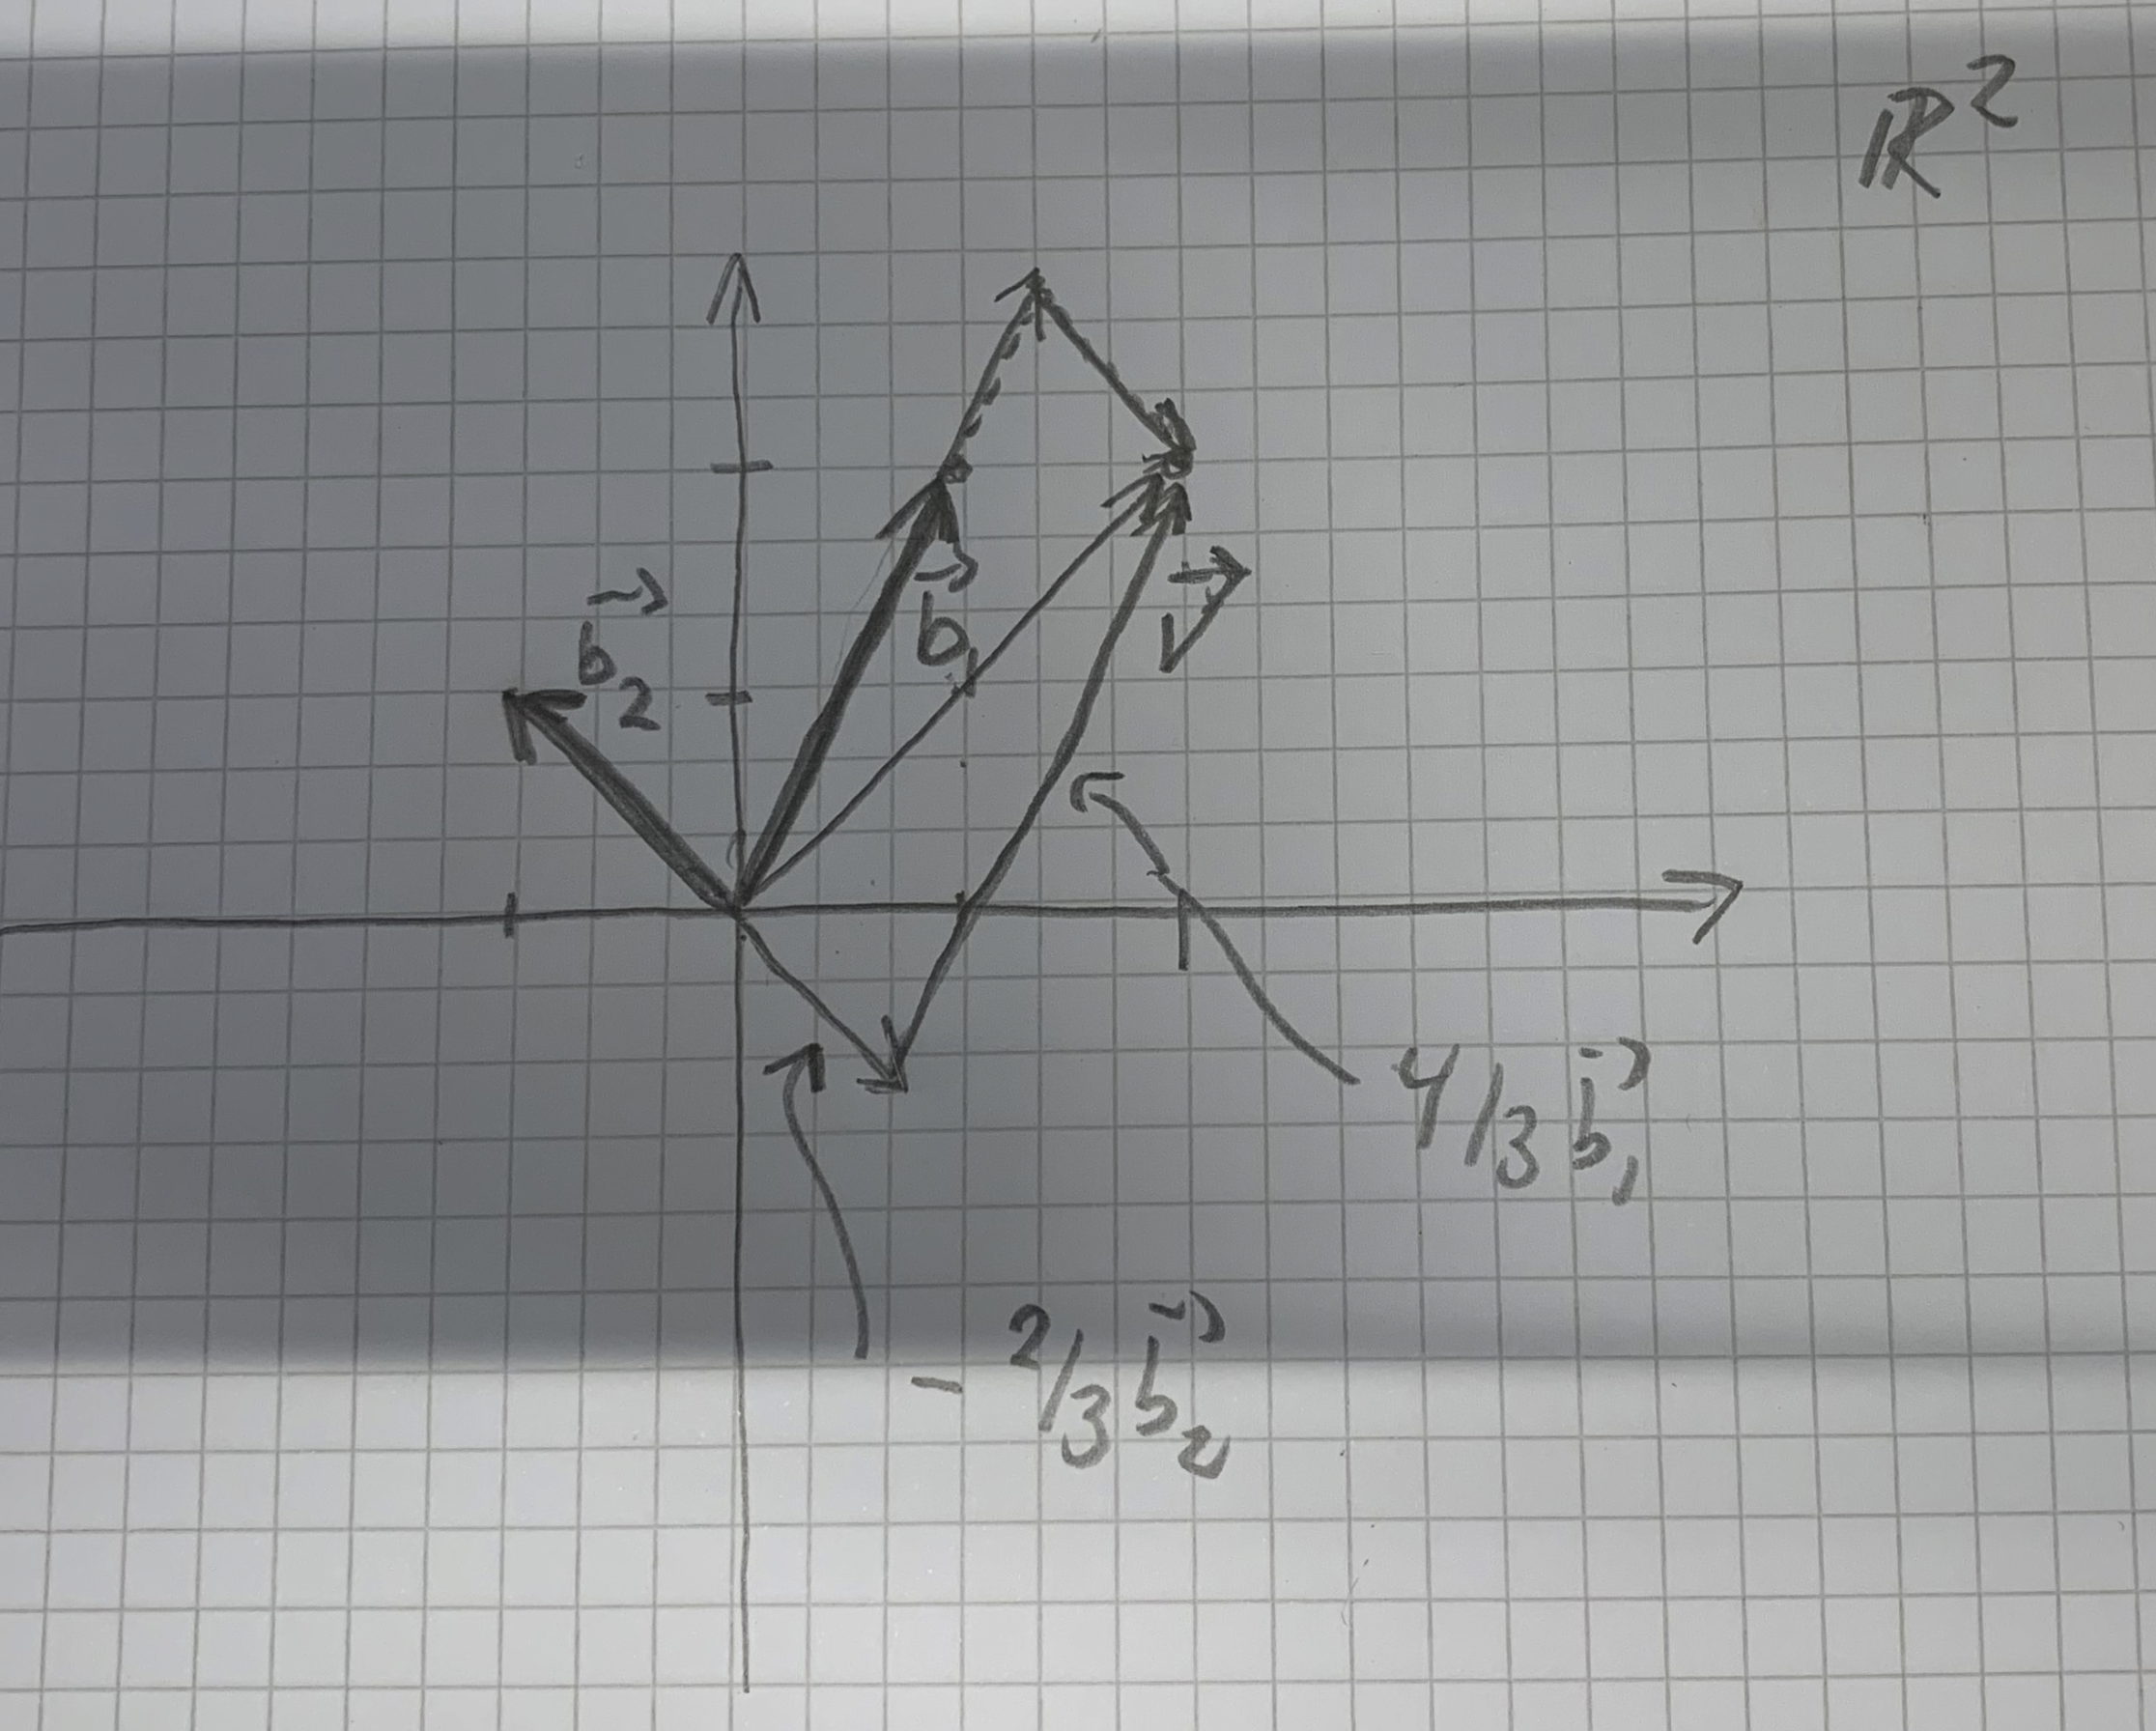
\includegraphics[width=6cm]{images/sol-fig1.png}

\end{solution}
\item\mytag{recommended}
    A person walks from home. First, they walk to the subway station. This is 1 km north and 500 m east as the crow flies. The subway takes the person to the city centre, which 3 km east and 2 km south of the subway station, as the crow flies. The person then walks 200 m south and 400 m west to their office.

    What are the coordinates of the office, relative to the person's home?

    What is the distance to home, as the crow flies?
    \begin{solution}
    The first point is solved by simple vector addition. The second point is by computing the euclidean norm.
    \end{solution}
\item
    A boat is sailing on the ocean, at a constant speed 20 km/h relative to the water surface, in the northeast direction. However, the water surface is moving too, at a constant velocity. After two hours, the boat is located 20 km north and 10 km east of the starting point. What is the speed and direction of ocean drift?
    \begin{solution}
        Using Pythagoras, we find that the velocity vector of the boat relative to the water surface is $\mathbf{v} = (\sqrt{2}/2)[20,20]^T$. The distance traveled relative to the water surface in two hours is $2\mathbf{v} = \sqrt{2}[20,20]^T$. The drift velocity is $\bvec{u} = [u_1,u_2]^T$. Over tho hours, $2\bvec{u}$. The total distance traveled relative to starting point is $2 \mathbf{v} + 2\bvec{u} = [10, 20]^T$. We get
        \[ \bvec{u} = [5,10]^T - \sqrt{2}[20,20]^T = [5-20\sqrt{2},10-20\sqrt{2}]^T. \]
        Using trig, the angle that $\bvec{u}$ makes with the west/east axis is
        \[ \theta = \tan^{-1} (u_2/u_1) \approx ... \]
        and the speed is the norm of $\|u\| \approx ... $.
    \end{solution}
\item  (Robert Beezer) A three-digit number has two properties. The tens-digit and the ones-digit add up to
5. If the number is written with the digits in the reverse order, and then subtracted from the original number,
the result is 792. Use a system of equations to find all of the three-digit numbers with these properties.
\begin{solution}
Let $a$ be the hundreds digit, $b$ the tens digit, and $c$ the ones digit. Then the
first condition says that $b + c = 5$. The original number is $100a + 10b + c$, while the reversed number is
$100c + 10b + a$. So the second condition is
$792 = (100a + 10b + c) - (100c + 10b + a) = 99a - 99c$.
So we arrive at the system of equations
$b + c = 5$, $99a - 99c = 792$.
By elementary row operations, we arrive at the equivalent system
$a - c = 8$, $b + c = 5$.
We can vary $c$ and obtain infinitely many solutions. However, $c$ must be a digit, restricting us to ten values
$(0 - 9)$. Furthermore, if $c > 1$, then the first equation forces $a > 9$, an impossibility. Setting $c = 0$, yields
$850$ as a solution, and setting $c = 1$ yields $941$ as another solution.
\end{solution}
\end{enumerate}

\section{More vectors and matrices}


These exercises are to get practice with computing matrix-matrix products, and to get an intuitive feel for them.
\begin{enumerate}
    \item \mytag{recommended} Let 
    \begin{equation}
        A = \begin{bmatrix} 1 & 3 \\ 0 & -2 \end{bmatrix}, \quad B = \begin{bmatrix} 7 & -1 & 0 \\ 8 & 1 & -1 \end{bmatrix}, \quad C = \begin{bmatrix} 0 & -1 \\ 5 & 7 \\ 0 & 7 \end{bmatrix}
    \end{equation}
    Which matrix products between pairs of these matrices are defined? Compute the products.
    \item\mytag{recommended} 
    Let $A$ be the $n\times n$ matrix defined by $A_{i,i+1} = i^2$ for $1 \leq i < n$, and zero otherwise. Compute the action of $A$ and $A^T$ on the standard basis for $\RR^n$. Compute the action of $A$ and $A^T$ on an arbitrary vector $\bvec{x}\in \RR^n$.
    \item
    Let $A \in M(n,m,\FF)$, $B \in M(n,o,\FF)$. Write $B$ in terms of column vectors, $B = [\bvec{b}_1,\cdots,\bvec{b}_o]$. Prove that
    \begin{equation}
        AB = [A\bvec{b}_1, \cdots, A\bvec{b}_o],
    \end{equation}
    i.e., $A$ acts on each individual column of $B$.     
    Similarly, show that, if we write $A$ in terms of its \emph{row vectors},
    \begin{equation}
        A = \begin{bmatrix} \bvec{a}_1^T \\ \bvec{a}_2^T \\ \cdots \\ \bvec{a}_n^T \end{bmatrix},
    \end{equation}
    then
    \begin{equation}
        AB = \begin{bmatrix} \bvec{a}_1^T B \\ \bvec{a}_2^T B \\ \cdots \\ \bvec{a}_n^T B  \end{bmatrix}.
    \end{equation}
    \item Show that the columns of $C = AB$ is a linear combination of the columns of $A$ with coefficients determined by $B$, 
    \begin{equation}
        \bvec{c}_i = \sum_j \bvec{a}_j B_{ji}
    \end{equation}
    Show a similar result for the rows of $C$.    
\end{enumerate}

\section{The complex numbers as a real vector space}

\begin{solution}
    This exercise is not essential, so can be skipped for most students.
\end{solution}
\mytag{for the curious}

The geometrical interpretation of the $\CC$ as the plane $\RR^2$ indicates that $\CC$ can be viewed as a two-dimensional real vector space. Indeed, addition and multiplication with \emph{real} scalars are compatible with the axioms for Euclidean space $\RR^2$.
\begin{enumerate}
    \item Show that $\CC$ regarded can be regarded as the Euclidean plane: Check axioms for Euclidean space and check that vector addition and multiplication with real scalars are the same in the two spaces. Check also that the Euclidean norm is the modulus of the complex number. What are the complex numbers that correspond to the standard basis in $\RR^2$? Conclude that $\CC$ can be regarded as a \emph{real} Euclidean vector space of dimension $2$.
    \begin{solution}
    The standard basis of $\RR^2$ corresponds to $1$ and $\rmi$. 
    \end{solution}
    \item Show that multiplication with a \emph{complex} number $z$ is a linear operator on $\RR^2$, and find its matrix in the standard basis. What is the matrix of multiplication with $\rmi$?
    \begin{solution}
    \[ (a + \rmi b)(x \rmi y) = (ax - by) + \rmi(ay + bx) \]
    We must find a matrix $A$ such that
    \[ A\begin{bmatrix} x\\y\end{bmatrix} = \begin{bmatrix} ax - by \\ bx + ay \end{bmatrix} \]
    The solution is
    \[ A = \begin{bmatrix}
        a & -b \\ b & a.
    \end{bmatrix} \]
    \end{solution}
    \item Show that multiplication with a complex number of modulus 1 is a rotation in $\RR^2$.
    \begin{solution} Strictly speaking, Euler's formula $e^{\rmi \theta} = \cos\theta + \rmi\sin\theta$ has not been introduced, so ``cannot'' be used here. But a complex number of modulus $1$ forms an angle $\theta$ with the $x$-axis. Since complex multiplication now will not change the length of $z$, only add the angles, this is a rotation. \end{solution}
    \item Show that the map $z \mapsto \bar{z}$ is a linear transformation in $\RR^2$. What kind of linear transformation is this? Is it a linear transformation in $\CC$?
\end{enumerate}

\section{Elementary row operations and Gaussian elimination}


\begin{enumerate}
\item
    Compute the overlap matrix $S$ of the basis in Eq.~\eqref{eq:1}. Use gaussian elimination to compute the inverse of the matrix $S$.
    
\begin{solution}
    The overlap matrix $S$ has elements $S_{ij} = \braket{\mathbf{b}_i,\mathbf{b}_j} =  \mathbf{b}_i^T \mathbf{b}_j$. We get
    \begin{equation}
        S_{11} = [1, 2] [1,2]^T = 1 + 4 = 5.
    \end{equation}
    \begin{equation}
        S_{22} = [-1, 1] [-1,1]^T = 2.
    \end{equation}
    \begin{equation}
        S_{21} = S_{12} = [1, 2] [-1,1]^T = -1 + 2 = 1.
    \end{equation}
    \begin{equation}
        S = \begin{pmatrix} 5 & 1 \\ 1 & 2 \end{pmatrix}
    \end{equation}
    To compute the inverse, we write down the augmented matrix
    \begin{equation}
        \begin{pmatrix} 5 & 1 & 1 & 0 \\ 1 & 2 & 0 & 1 \end{pmatrix}
    \end{equation}
    Divide row 1 by 5 and subtract from the second row:
    \begin{equation}
        \begin{pmatrix} 1 & 1/5 & 1/5 & 0 \\ 0 & 9/5 & -1/5 & 1 \end{pmatrix}
    \end{equation}
    Divide second row by 9,
    \begin{equation}
        \begin{pmatrix} 1 & 1/5 & 1/5 & 0 \\ 0 & 1/5 & -1/45 & 1/9 \end{pmatrix}
    \end{equation}
    Subtract row 2 from row 1,
    \begin{equation}
        \begin{pmatrix} 1 & 0 & 10/45 & -1/9 \\ 0 & 1/5 & -1/45 & 1/9 \end{pmatrix}
    \end{equation}
    Multiply row 2 by 5:
    \begin{equation}
        \begin{pmatrix} 1 & 0 & 10/45 & -1/9 \\ 0 & 1 & -1/9 & 5/9 \end{pmatrix}
    \end{equation}
    We can now read off $S^{-1}$ from the right block:
    \begin{equation}
        S^{-1} = \begin{pmatrix}  10/45 & -1/9 \\  -1/9 & 5/9 \end{pmatrix}
    \end{equation}
\end{solution}

\item    
    Write down the dual basis of $B = \{\mathbf{b}_1,\mathbf{b}_2\}$.
\item\mytag{recommended} (Robert Beezer)  Consider the following system of equations:
\begin{align}
    2 x_1 -3x_2 + x_3 + 7 x_4 &= 14\\
    2x_1 + 8x_2 - 4x_3 + 5x_4 &= -1\\
    x_1 + 3x_2 - 3x_3 &= 4\\
    -5 x_1 + 2x_2 + 3 x_3 + 4x_4 &= -19
\end{align}
Use gaussian elimination to find all possible solutions. Write down the set of all solution using set notation.
\begin{solution}
    Using elementary operations, we get the augmented matrix
    \[ \begin{bmatrix} 1 & 0 & 0 & 0 & 1 \\ 0 & 1 & 0 & 0 & -3 \\ 0 & 0 & 1 & 0 & -4 \\ 0 & 0 & 0 & 1 & 1 \end{bmatrix} \]
    The solution is unique, and given by $x_1 = 1$, $x_2 = -3$, $x_3 = -4$, and $x_4 = 1$. The solution set is
    \[ S = \{ [1,-3,-4,]^T \} \]
\end{solution}
\item(Robert Beezer) Find all possible solutions of the linear system
\begin{align}
    3 x_1 + 4 x_2 - x_3 + 2 x_4 &= 6 \\
    x_1 - 2 x_2 + 3 x_3 + x_4 &= 2 \\
    10 x_2 - 10 x_3 - x_4 &= 1
\end{align}
Write down the solution set using set notation.
\begin{solution}
    By elementary row operations, we obtain the augmented matrix:
    \[ \begin{bmatrix} 1 & 0 & 1 & 4/5 & 0 \\ 0 & 1 & -1 & -1/10 & 0 \\ 0 & 0 & 0 & 0 & 1 \end{bmatrix} \]
    The last row represents the equation  $0=1$, so there cannot be a solution to the system. $S = \{ \} = \emptyset$.
\end{solution}
\item (Robert Beezer) Find all possible solutions of the linear system
\begin{align}
    2 x_1 + 4 x_2 + 5 x_3 + 7 x_4 &= -26 \\
    x_1 + 2x_2 + x_3 - x_4 &= -4 \\
    -2 x_1 - 4 x_2 + x_3 + 11 x_4 &= -10
\end{align}
Write down the solution set using set notation.
\begin{solution}
The augmented matrix reduces to
\[ \begin{pmatrix} 1 & 2 & 0 & -4 & 2 \\ 0 & 0 & 1 & 3 & -6 \\ 0 & 0 & 0 & 0 & 0 \end{pmatrix} \]
The last row corresponds to the equation $0=0$, so this is ok. The two first rows correspond to infinitely many solutions. The second row is equivalent to
\[ x_3 = -3 x_4 - 6.\]
This expresses $x_3$ in terms of $x_4$. The first row becomes the equation
\[ x_1 = -2x_2 + 4x_4 + 2.\]
We see that we obtain a solution for any choice of $x_2$ and $x_4$. The set of solutions is
\[ S = \{ [-2 x_2 + 4 x_4 + 3, x_2, -3 x_4 - 6, x_4]^T \mid x_2,x_4 \in \FF\} \]
\end{solution}
\end{enumerate}



\begin{enumerate}[resume]
    \item 
    Let $\mathbf{b}_i$, $i=1,2,\cdots,n$ be a basis for $\RR^n$. Let 
    \[ B = [\mathbf{b}_1, \mathbf{b}_2, \cdots, \mathbf{b}_n] \]
    be the \emph{basis matrix}, whose columns are precisely the $\mathbf{b}_i$. Explain that if $\mathbf{y} = x_1 \mathbf{b}_1 + \cdots + x_n \mathbf{b}_n$, then
    \[ B \mathbf{x} = \mathbf{y}. \]
    Solve for $\mathbf{x}$ using $B$ in symbols.
    \begin{solution}
        We know that the overlap matrix should be key here. So we multiply with $B^T$ from the left to get $B^T B \bvec{x} = B^T \bvec{y}$. Thus,
        \[ \bvec{x} = S^{-1} B^T \bvec{y}. \]
        We know that the overlap matrix $S = B^T B$ is invertible, since $B$ is a basis matrix.
    \end{solution}
\item
    Let $n$ linearly independent vectors $B = \{\mathbf{b}_1, \cdots,\mathbf{b}_n\}$ of $\FF^n$ be given. Write down a formula for the dual basis in terms of the overlap matrix.
    \begin{solution}
        The dual basis $\tilde{B} = [\tilde{\bvec{b}}_1, \cdots \tilde{\bvec{b}}_n]$ is such that $\braket{\tilde{\bvec{b}}_i,\bvec{b}_j} = \delta_{ij}$. We obtain the equation
        \[ \tilde{B}^H B = I. \]
        Thus,
        \[ \tilde{B} = (B^{-1})^H. \]
    \end{solution}
\end{enumerate}


\begin{solution}
    Consider the system
    \begin{equation}
        B \mathbf{x} = \mathbf{v}.
    \end{equation}
    Here, $B = [\mathbf{b}_1, \mathbf{b}_2]$ is the matrix that has the basis vectors as columns. This system is precisely what we solved above in the two-dimensional case.

    We multiply by $B^T$ to get
    \[ S \mathbf{x} = B^T \mathbf{v}. \]
    We invert $S$ to get
    \[ \mathbf{x} = S^{-1} B^T \mathbf{v}. \]
\end{solution}



\section{Bra-ket notation}
\begin{solution}
    I think it is important that the students try to relate bra-ket notation to more standard linear algebra notation.
\end{solution}

\begin{enumerate}
\item
    Let a basis $B = \{b_1, b_2,\cdots, b_n\}$ be a basis for a finite-dimensional Hilbert space, and let $\{\ket{i}\}$ be a the standard basis for $\CC^n$. Consider the operator defined by
    \begin{equation}
        \hat{B} = \sum_{i=1}^n \ket{b_i} \bra{i},
    \end{equation}
    What is the domain of $\hat{B}$, and the range of $\hat{B}$? In other words, which spaces does $\hat{B}$ map from and to?
    \begin{solution}
        The domain is $\CC^n$, and the range is $V$. It takes vectors in $\CC^n$ and moves them to $V$.
    \end{solution}
\item
    Let $\ket{x} \in \CC^n$, and consider
    \[ \ket{\psi} = \hat{B} \ket{x}. \]
    Can you interpret this expression in terms of bases and expansion coefficients?
    \begin{solution}
        The components $x_i = \braket{i|x}$ are the expansion coefficients of $\ket{\psi}$ in the basis $B$. 
    \end{solution}
\item
    Show that
    \begin{equation}
        \hat{S} = \sum_{ij} \ket{i} \braket{{b}_i|{b}_j} \bra{j}.
    \end{equation}
    This is the overlap matrix expressed as an operator.
    Find an expression for the basis coefficients $x_i$ in terms of the basis alone.
    \begin{solution}
        $\ket{x} = \hat{S}^{-1} \hat{B}^\dag \ket{\psi}$. 
    \end{solution}
\end{enumerate}


\section{Eigenvalue decomposition}

\begin{solution}
{\bfseries Tutor note:} This exercise may be considered for the especially interested student. It requires some mathematical argument skill. I would not consider it \emph{hard}, though, but perhaps not focus on this exercise to begin with. I will try to make a solution for this in time.
\end{solution}

\mytag{for the curious}

Of great importance to quantum chemistry is the time-independent Schr\"odinger equation: Given the Hamiltonian operator $\hat{H}$, which is usually Hermitian, find a nonzero $\ket{\psi}$, called an eigenvector, and a real number $E$, called an eigenvalue, such that
\begin{equation}
    \hat{H} \ket{\psi} = E \ket{\psi}.
\end{equation}
Choosing a particular orthonormal basis $\{\ket{\phi_i}\}$ for Hilbert space, a matrix eigenvalue problem arises,
\begin{equation}
    A \bvec{u} = E \bvec{u}, \quad u_i = \braket{\phi_i|\psi}, \quad A_{ij} = \braket{\phi_i|\hat{H}|\phi_j}.
\end{equation}

We prove the spectral theorem for normal operators over finite dimensional Hilbert spaces. The spectral theorem states that one can actually find a \emph{basis} of eigenvectors for normal operators. The normal operators include the Hermitian operators.

In this section, we let $M(n) = M(n,n,\CC) = \CC^{n\times n}$ be the set of complex square matrices of dimension $n$.


Two matrices $A$ and $B$ are said to be \emph{similar} if there is an invertible matrix $U$ such that $A = U B U^{-1}$. If $U$ is unitary, then $A$ and $B$ are \emph{unitarily similar}. ($U$ is unitary if and only if $U^H = U^{-1}$.)

\begin{enumerate}
\item
    What does it mean that $A \in M(n)$ is normal?
\item   
    Prove that a diagonal matrix $D \in M(n)$ is normal. (A matrix $A$ is diagonal if and only if $A_{ij}=0$ whenever $i\neq j$.)
    \item Prove that $U$ is unitary if and only if its columns are orthonormal.
\item \label{item:needed} Prove that if $A$ is a normal matrix, if $B$ is unitarily equivalent to $A$, then $B$ is normal. 
\item Prove that if $A$ is unitarily equivalent to a diagonal matrix,  then $A$ is normal.
\end{enumerate}

The next part requires \emph{Schur's Lemma}:
\begin{myLemma}{Schur's Lemma}{}
Let $A \in M(n)$. Then $A$ is unitarily equivalent to an upper triangular matrix. ($R$ is upper triangular if $R_{ij}=0$ whenever $i > j$.)
\end{myLemma}
The proof of Shur's Lemma can be found in, e.g., Fraleigh and Beauregard.

\begin{enumerate}[resume]
\item Prove that every normal matrix $A$ is unitarily equivalent to a normal upper-triangular matrix $B$. (Use Schur's Lemma and exercise \ref{item:needed}.)
\item Prove that a normal upper triangular matrix $B$ must be diagonal. Hint: Let $C = B^H B = BB^H$, and compute $C_{11}$ to show that $B_{1j} = 0$ if $j > 1$. Continue to $C_{22}$, and all the way up to $C_{nn}$.
\end{enumerate}

We have now proved:
\begin{myTheorem}{Spectral theorem for normal matrices}{}
    Suppose $A \in M(n)$ is normal, i.e., $AA^H = A^H A$. Then there is a unitary matrix $U \in M(b)$ and a diagnal matrix $D \in M(n)$ such that
    \begin{equation}
        A = U D U^H. \axiomname{spectral decomposition}
    \end{equation}
\end{myTheorem}

\begin{enumerate}[resume]
    \item Let $\mathbf{u}_i = U_{:.i}$ be the $i$th column for $U$. Explain why these vectors form a basis for $\CC^n$.
    \item Show that
    \begin{equation}
        A = \sum_{i=1}^n d_i \mathbf{u}_i \mathbf{u}_i^H, \quad d_i = D_{ii}. \axiomname{spectral decomposition}
    \end{equation}
    Write this formula also using bra-ket notation.
    \item
        What does $A$ do with the vector $\bvec{u}_k$ for some $k$? What does $A$ do to a linear combination of the basis vectors?
\end{enumerate}

A special kind of normal matrix is the Hermitian matrix:
\begin{equation}
    A^H = H.
\end{equation}
\begin{enumerate}[resume]
    \item Show that a Hermitian matrix is unitarily equivalent to a diagonal matrix with \emph{real} numbers on the diagonal, i.e., $A = U D U^H$ with $D_{ii} \in \RR$.
\end{enumerate}

\section{Diagonalization of a matrix}

\begin{solution}
{\bfseries Tutor note:} This exercise, I find quite important for understanding eigenvalue problems. I therefore recommend it. The students could also use computations in Python or similar if they find the analytic part a little hard.

I think this is one of th exercises that the tutors should spend some time with.
\end{solution}


A matrix $A$ has an eigenvalue $E$ if and only if there is a nonzero solution to the linear system
\[ (A - EI)\bvec{x} = 0. \]
Thus, the matrix $A - EI$ must be singular, i.e., not invertible. The eigenvector $\bvec{x}$ is then a vector in the null space of this matrix.

A sufficient and necessary criterion for invertibility of a matrix $B$ is that the \emph{determinant} is nonzero. The definition of the determinant can be stated as follows:
\begin{myDefinition}{Determinant}{}
Let $A \in M(n)$. The determinant, written $\det(A) \in \CC$ is defined by
\begin{equation}
    \det(A) = \sum_{p \in S_n} (-1)^{|p|} A_{1,p(1)} A_{2,p(2)} \cdots A_{n,p(n)}.
\end{equation}
Here, $S_N$ is the set of \emph{permutations} of the numbers $\{1,2,\cdots,n\}$. A permutation is by definition any bijective map.
\end{myDefinition}


Each permutation $p \in S_n$ is a rearrangement is thus completely specified by the new order of the numbers $\{1,2,\cdots,n\}$, i.e., $(p(1),p(2),\cdots,p(n))$. For example, $(1,2,3,4,5,6) \in S_6$ is the \emph{identity permutation} that leaves any number alone. The permutation $(3,2,1,4,6,5)$ makes 1 and 3 switch place, and 5 and 6.

Any permutation can be written as a product (composition) of \emph{transpositions}, i.e., switching of exactly two elements. Thus, $(3,1,2) = (1,2)(2,3)$. Here, the two-element notation indicates which elements are swithced. It is a fact that all permutations can be decomposed in \emph{either} an even number of permutations, or an odd number of permutations, denoted $|p|$. The \emph{sign} of a permutation $p$ is $(-1)^{|p|}$, and is unique for a permutation.

There are $n!$ unique permutations of an $n$-element set.

\begin{enumerate}
    \item Write out the set of permutations $S_1$, $S_2$ and $S_3$. 
    \item 
    Compute the sign of the permutations of the previous exercise.
    \item Compute explicit expressions for the determinants of matrices of dimension 1, 2, and 3.
    \item (Extra.) In Python, the module \texttt{itertools} contains an iterator class \texttt{permutations} that allow efficient looping over permutations. Can you write a function that computes the sign of a permutation? Use the internet for efficiency. 
    \item  Compute explicit expressions for the determinants of matrices of dimension up to 3. By equating the determinant of $A - EI$ with zero, a polynomial equation in $E$ is obtained. Find the solutions in the case $n=2$.
    \item Consider the matrix
    \[ A = \begin{bmatrix} -1 & z \\ z & 1 \end{bmatrix} .\]
    For which $z \in \CC$ is $A$ Hermitian? Normal? Compute the eigenvalues as function of $z$. Also find the eigenvectors.
    \item  For which values of $z$ does there exist a basis of eigenvectors?
\end{enumerate}

\section{Gram--Schmidt orthogonalization}

\begin{solution}
{\bfseries Tutor note:}
I think Gram--Schmidt is important, but maybe there is not enough time in the exercise session.

This exercise \emph{may} be a little hard for some students, because it requires some ``proving.'' On the other hand, if there are students that want do do it, the tutors should be prepared ... 
\end{solution}

\mytag{for the curious}
Let $V$ be a vector space over $\FF$ with $\dim(V) = n < +\infty$. Recall that every finite-dimensional vector space has a basis. In the lecture notes, it is claimed that every finite dimensional Hilbert space has a basis of orthonormal vectors! Recall, that in an orthonormal basis, computations are usually much simpler than in nonorthogonal bases.

In this exercise, we show that any set of linearly independent vectors can be orthonormalized. We work in the space $\FF^n$ for simplicity. That is, let $B = [\bvec{b}_1,\cdots,\bvec{b}_m]\subset \FF^n$ be a set of $m \leq n$ linearly independent vectors, spanning a subspace $V = \spn(B)$. We denote the vector set by its basis matrix $B$. Equivalently, $B$ is an arbitrary matrix in $M(n,m,\FF)$ of full rank $m$, and the vectors $\bvec{b}_i$ are the columns of $B$.

We will find a set of orthonormal vectors $U = [\bvec{u}_1,\cdots,\bvec{u}_m]$, again denoted by a matrix in $M(n,m,\FF)$, such that $\spn(B) = \spn(U)$. That is, the two sets of vectors are bases for the \emph{same} subspace, but one of them is an orthonormal basis.

We first define the notion of orthogonal projection onto the span of a single vector: Let $\bvec{y}\in \FF^n$ be nonzero, $Y = \spn(\bvec{y})$, and let $\bvec{x} \in \FF^n$.
\begin{enumerate}
    \item Show that the vector $\bvec{x}_Y$ given by
    \begin{equation}
        \bvec{x}_Y = \bvec{y}\frac{\braket{\bvec{y}, \bvec{x}}}{\braket{\bvec{y},\bvec{y}}} 
    \end{equation}
    is the \emph{unique} vector in $Y$, such that
    \begin{equation}
        \forall \bvec{y}' \in Y, \quad \|\bvec{x} - \bvec{x}_Y\| \leq \|\bvec{x} - \bvec{y}'\|.
    \end{equation}
    Hint: Find a function $f : \RR \to \RR$ which you can study, by using the definition of $Y = \spn(\bvec{y})$.
    \item
    Show that
    \begin{equation}
        \bvec{x} = \bvec{x}_Y + \bvec{x}_{Y^\bot},
    \end{equation}
    where
    \begin{equation}
        \braket{\bvec{x}_{Y^\bot}|\bvec{x}_Y} = 0.
    \end{equation}
    Illustrate with a picture of the situation in $\RR^2$.
\end{enumerate}
The vector $\bvec{x}_Y$ is called the \emph{orthogonal projection of $\bvec{x}$ onto $Y$ or $\bvec{y}$}.
\begin{enumerate}[resume]
\item Explain that the orthogonal projection is given by acting with an operator, 
\begin{equation}
    \bvec{x}_Y = P_\bvec{y} \bvec{x}, \quad P_{\bvec{y}} = \bvec{y} \braket{\bvec{y},\bvec{y}}^{-1} \bvec{y}^H.
\end{equation}
The operator $P_{\bvec{y}}$ 
is called the \emph{orthogonal projection operator onto $Y$ or  $\bvec{b}$}.
\end{enumerate}

\begin{enumerate}[resume]
\item Show that $P^2 = P$ and that $P^\dag = P$.
\end{enumerate}
The Gram--Schmidt orthogonalization proceeds recursively:
\begin{enumerate}[label=\arabic*.]
    \item $\bvec{u}_1 = \bvec{b}_1 \braket{\bvec{b}_1,\bvec{b}_1}^{-1/2}$ (normalization)
    \item $\bvec{u}_2' = \bvec{b}_2 - P_{\bvec{u}_1} \bvec{b}_2$ (removal of projection), and $\bvec{u}_2 = \bvec{u}_2' \braket{\bvec{u}_2',\bvec{u}_2'}^{-1/2}$ (normalization)
    \item $\bvec{u}_3' = \bvec{b}_3 - P_{\bvec{u}_1} \bvec{b}_3-P_{\bvec{u}_2} \bvec{b}_3$ (removal of projection), and $\bvec{u}_3 = \bvec{u}_3' \braket{\bvec{u}_3',\bvec{u}_3'}^{-1/2}$ (normalization)
    \item \ldots
    \item $\bvec{u}_m' = \bvec{b}_m - \sum_{i=1}^m P_{\bvec{u}_i} \bvec{b}_m$ (removal of projection), and $\bvec{u}_m = \bvec{u}_m' \braket{\bvec{u}_m',\bvec{u}_m'}^{-1/2}$ (normalization)
\end{enumerate}
We see that each $\bvec{u}_i$ is given by projecting away from $\bvec{b}_i$ the components of all the \emph{previously generated} $\bvec{u}_j$, $j<i$.

\begin{enumerate}
    \item Show that all the generated vectors $\bvec{u}_i$ are orthonormal.
    \item Show that a set of orthonormal vectors are linearly independent.
    \item Show that the span of the first $k$ original vectors is the same as the span of the first $k$ generated vectors.
    Show that
    \begin{equation}
        B = U R,
    \end{equation}
    where $R \in M(m,m,\FF)$ is \emph{upper triangular}, i.e., $R_{ij}=0$ whenever $i > j$.
    This is called the QR decomposition of the operator $B$. (The ``Q'' is just our $U$.)
    \item We have shown the existence of the QR decomposition when $B$ had full rank. Can you show the existence of the decomposition when $B$ does \emph{not} have full rank? It always exists. Hint: What happens when $B$ does not have full rank?
    \begin{solution} Sketch:
        When $B$ does not have full rank, say $m' < m$, there are $m-m'$ vectors that can be removed from $B$ due to linear dependence. Apply QR to this reduced $B$, and adjoin to $U$ two vectors orthogonal to all the $\bvec{u}_i$ generated, (they exist, but this must strictly speaking be proven) and zeroes to $R$.
    \end{solution}
\end{enumerate}


We now turn to a computational exercise:
\begin{enumerate}[resume]
\item Write a Python function to compute the QR decomposition of a matrix with full rank. In SciPy, the function \texttt{scipy.linalg.qr} is an advanced implementation with pivoting. To compare with your implementation, use the call
\begin{verbatim}
    Q,R = qr(A,mode='economic',pivoting=False)
\end{verbatim}
With \texttt{pivoting=False}, the function computes essentially the same as our presented algorithm. (Turning on pivoting stabilizes the algorithm, rearranging the vectors before orthogonalizing.)
\item Let $n\geq m>0$ be integers, and define the matrix $A\in \RR^{n\times m}$ by
\begin{equation}
    A_{ij} = \left(\frac{i-1}{n-1}\right)^{j-1}.
\end{equation}
This the matrix of the $m$ first monomials $x^{j-1}$ evaluated at an equidistant grid of $n$ points in the interval $[0,1]$.
Test your QR implementation on $A$ for various $n,m$, say $m=10$ and $m=200$. In particular, compute the difference between your factorization and $A$, and compare also with the NumPy implementation.
\end{enumerate}

% \section{More orthogonal projections}

% Let $V$ be of dimension $n < +\infty$ over $\FF$.
% We now study \emph{orthogonal projections}.

% \begin{definition}
%     Let $S \subset V$ be a linear subspace, and let $\ket{\psi}\in V$ be arbitrary. The \emph{orthogonal projection} of $\ket{\psi}$ onto $S$ is the unique vector $\ket{\psi_S}\in S$ such that for all $\ket{\phi}\in S$,
%     \begin{equation}
%         \| \ket{\psi} - \ket{\psi_S}\| \leq \|\ket{\psi} - \ket{\phi}\|
%     \end{equation}
%     Thus, the orthogonal projection is the best approximation in $S$ of $\ket{\psi}$, in the sense that the norm is minimized.
% \end{definition}

% We have to prove that such a best approximation exists, and that it is unique. For simplicity we consider the case $\FF=\RR$, but the complex case is similar.
% \begin{enumerate}
%     \item Let $U = [\ket{u_1},\cdots,\ket{u_m}]$ be an a basis for $S$, such that for any $\ket{\phi}\in S$ there is a unique $\ket{x}\in \FF^m$ such that $\ket{\phi} = U\ket{x}$. Why does $\ket{x}$ exist? Why is it unique?
%     \item Define the function $F : \FF^m \to \RR$ by
% \begin{equation}   
% F(x_1,\cdots,x_m) = \frac{1}{2}\|\ket{\psi} - U\ket{x}\|^2.
% \end{equation}
%     Show that the partial derivatives of $F$ are
%     \begin{equation}
%         \pdiff{F}{x_i} = \bra{u_i}(\ket{\psi} - U\ket{x}).
%     \end{equation}
%     \item Show that the equation $\pdiff{F}{x_i}=0$ is equivalent to solving the linear system
%     \begin{equation}
%         S \ket{x} = \ket{y}, \quad \ket{y} = U^\dag \ket{\psi}.
%     \end{equation}
%     Explain that this system has a unique solution. Conclude that there is only one critical point of $F$. Show that this critical point is a global minimum.
%     \item Let $\ket{\psi_\bot} = \ket{\psi} - \ket{\psi_S}$ be the error. Show that
%     \begin{equation}
%     \forall \ket{\phi}\in S, \quad        \braket{\phi|\psi_\bot} = 0
%     \end{equation}
%     and Pythagoras' law,
%     \begin{equation}
%         \|\ket{\psi}\|^2 = \|\ket{\psi_S}\|^2 + \|\ket{\psi_\bot}\|^2.
%     \end{equation}
% \end{enumerate}

% In the above exercise, we proved that any vector $\ket{\psi}$ has a unique decomposition into the orthogonal projection onto $S$ and the error, which is orthogonal to $S$. 

% \begin{definition}{Orthogonal projector}{}
% An \emph{orthogonal projector} is an operator $P \in L(V)$ such that (a) $P = P^\dag$ (Hermitian) and (b) $P^2 = P$ (idempotent).
% \end{definition}

% \begin{enumerate}
%     \item Explain why $P$ has $n$ linearly independent orthonormal eigenvectors. Show that the only possible eigenvalues are 0 and 1.
%     \begin{solution}
%     If $P\ket{u} = \lambda \ket{u}$, then $\lambda\in \RR$ since $P=P^\dag$. Since $P^2 = P$, we see that $P\ket{u} = \lambda^2 \ket{u}$. Hence, $\lambda = \lambda^2$, and thus either $\lambda = 0$ or $\lambda = 1$. Since $P$ is Hermitian, and hence normal, it has a complete set of eigenvectors.
%     \end{solution}
%     \item Show that there is an $m \leq n$ such that one can write
%     \begin{equation}
%     P = \sum_{i=1}^m \ket{u_i} \bra{u_i}, \label{eq:projector}
%     \end{equation}
%     where $P\ket{u_i} = \ket{u_i}$.

% \end{enumerate}

% Let $\ket{u}$ with $\|u\|=1$, and consider the one-dimensional subspace spanned by $\ket{u}$:
% \begin{equation}
%     S_{\ket{u}} = \operatorname{span}(\ket{u}) = \{ \alpha \ket{u} \mid \alpha \in \FF \}.
% \end{equation}
% (Imagine a line in Hilbert space.)
% The projection of a vector $\ket{\psi}\in V$ onto the line $S_{\ket{u}}$ is defined as the vector $\ket{\psi_0}\in S_{\ket{u}}$ that minimizes the distance to $S_{\ket{u}}$, i.e., $\ket{\psi_0} \in S_{\ket{u}}$ and 
% \begin{equation}
%    \forall \ket{\phi} \in S_{\ket{u}}, \quad \|\ket{\psi} - \ket{\psi_0}\| \leq \|\ket{\psi} - \ket{\phi}\|.
% \end{equation}
% \begin{enumerate}[resume]
% \item Show that $\ket{\psi}$ can be decomposed as \begin{equation}
%     \ket{\psi} = \ket{\psi_0} + \ket{\psi_\perp}, 
% \end{equation}
% where $\braket{u|\psi_\perp} = 0$. Thus, we have a decmposition into orthogonal vectors. Draw a picture that illustrates this.
% \item Define $P_{\ket{u}}\ket{\psi} = \ket{u} \braket{u|\psi}$. Show that $P_{\ket{u}}$ is a linear operator. Show that $P = P^\dag$ and that $P^2 = P$. Show that $\ket{\psi_0} = P_{\ket{u}}\ket{\psi}$.
% \end{enumerate}

% More generally, let $U = \{\ket{u_1},\cdots,\ket{u_m}\}$ be a set of $m$ orthonormal vectors. They are linearly independent, and therefore define a linear subspace $S_U$ defined by all possible linear combinations, the span of $U$.

% The orthogonal projection of $\ket{\psi}$ onto $U$ is again the vector that minimizes the distance to $S_U$.

% \begin{enumerate}[resume]
% \item Show that the orthogonal projection onto $S_U$ is given by the operator in Eq.~\eqref{eq:projector}.
% \item Suppose that $U'$ is a different orthonormal basis for $S_U$. Show that there exists a unitary $X \in M(m)$ such that $U' = UX$. 
% \item Show that the projector expression~\eqref{eq:projector} is independent of basis, i.e.,
% \[ P = \sum_{i=1}^m \ket{u_i} \bra{u_i} = \sum_{i=1}^m \ket{u'_i} \bra{u'_i}. \]
% \end{enumerate}

% We now generalize to non-orthonormal bases. Let $B = [\ket{b}_1,\cdots,\ket{b}_m] = \sum_i^m \ket{b_i}\bra{i}$ be a linearly independent set, but not necessarily orthonormal. Let $S = B^\dag B$ be the overlap matrix. 
% \begin{enumerate}[resume]
% \item Recall the dual basis. Show that
% \begin{equation}
%     P = \sum_{i=1}^m \ket{b_i} \bra{\tilde{b}_i}
% \end{equation}
% is an orthogonal projector.
% \item In what way are the bases $B$, $\tilde{B}$, and $U = [\ket{u_1},\cdots,\ket{u_m}]$ from Eq.~\eqref{eq:projector} related?
% \end{enumerate}


\section{The singular value decomposition as a compression tool}

\begin{solution}
    {\bfseries Tutor note:} This exercise is very nice, in my opnion, with a mix of computations and not-so-hard analysis. However, it will probably take the best part of an hour, if not more, depending on the student.
\end{solution}

\mytag{for the curious} 

The SVD is a very powerful linear algebra tool. In quntum chemistry it is used to compress electron repulsion integrals, for example.

In this small exercise, we demonstrate its power applied to \emph{image compression}. For this exercise, a good grayscale image is handy. You can find a nice picture of a parrot in Figure~\ref{fig:parrot}.

Recall first the \emph{Hilbert--Schmidt} inner product on the set $M(n,m,\FF)$ of matrices:
\begin{equation}
    \braket{X,Y}_\text{HS} = \Tr (X^H Y) 
\end{equation}
The \emph{trace} $\Tr(A)$ is the sum of the diagonal elements of $A$.

Recall also the SVD: For $A \in M(n,m,\FF)$, and $k = \min(n,m)$, there are unitary matrices $U \in M(n)$ and $V\in M(m)$, such that $U^H U = I_n$ and $V^H V = I_m$, and numbers$\sigma_1 \geq \sigma_2 \geq \cdots \sigma k$, such that
\begin{equation}
    A = U \Sigma V^H = \sum_{i=1}^k \bvec{u}_i \sigma_i \bvec{v}_i^H,
\end{equation}
where $\Sigma \in M(n,m,\RR)$ is such that the upper $k\times k$ block is diagonal, with the $\sigma_i$s along the diagonal, and the rest is zero. Note that $U$ and $V$ may have columns that do not enter the expansion on the right-hand side. Thus, the ``full SVD'' on the left hand side can be reduced to the ``economical SVD'',
\begin{equation}
    A = U \Sigma V = U_{:,:k} \Sigma_{:k,:k} V_{:,:k}^H,
\end{equation}
where the index ``$:k$'' is short for the selection of the $k$ first indices, and ``$:$'' is everything.

\begin{figure}
    \centering
    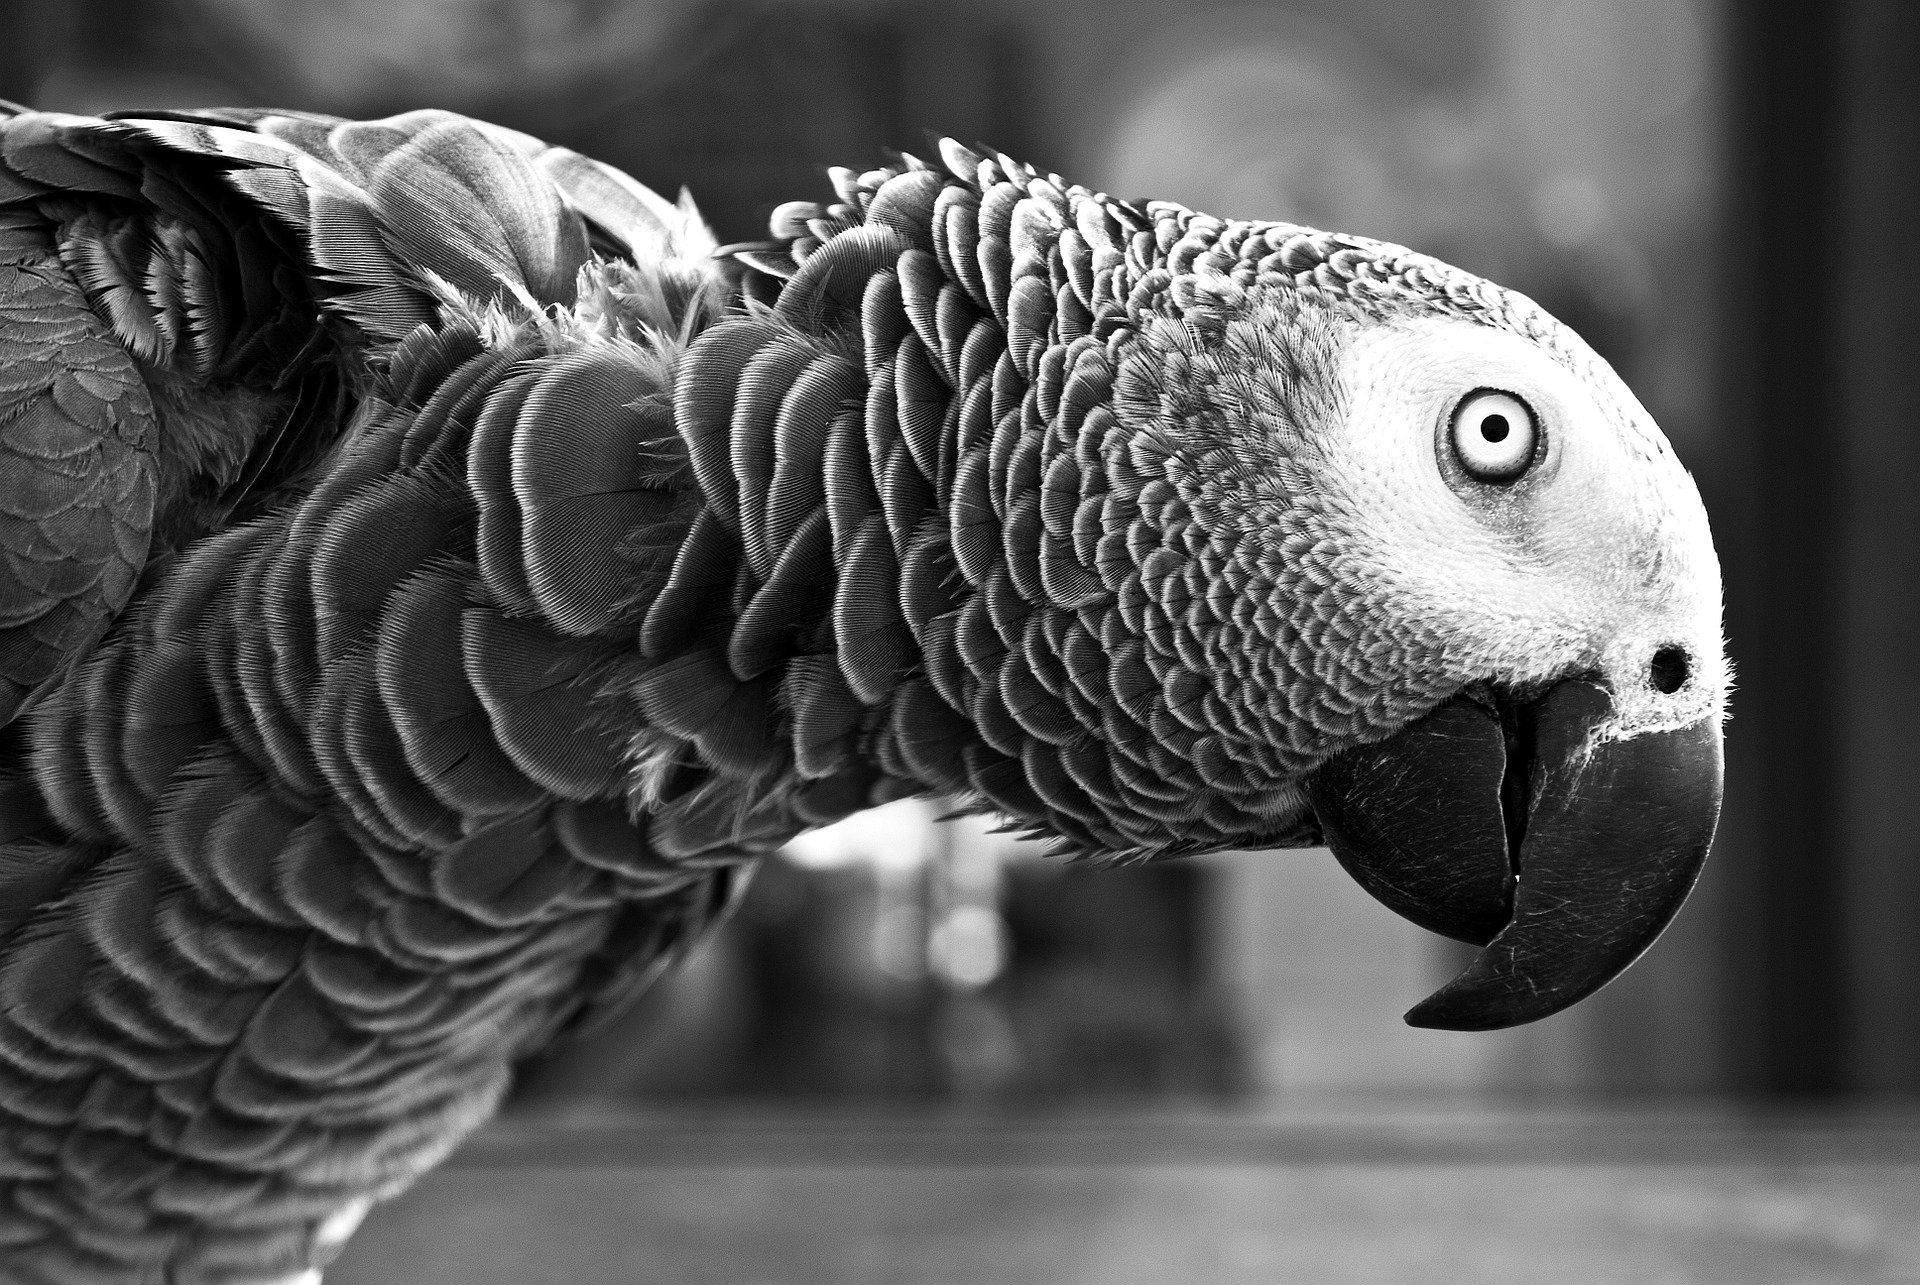
\includegraphics[width=0.75\textwidth]{images/parrot.jpg}
    \caption{A parrot, \url{https://www.dropbox.com/s/8r4svs6uuhgwawt/parrot.png} }
    \label{fig:parrot}
\end{figure}

\begin{enumerate}
    \item How is the Hilbert--Schmidt inner product related to the Euclidean inner product and the standard Euclidean vector space?
    \item Show that $\Tr(ABC) = \Tr(CAB)$ (cyclic invariance).
    \item Let $\bvec{u}_i$ and $\bvec{v}_i$ be the left and right singular vectors of a matrix $A$. Show that the matrices $X^{ij} = \bvec{u}_i\bvec{v}_j^T$  form an orthonormal set in the Hilbert--Schmidt inner product.
    \begin{solution}
    \begin{equation*}
    \braket{X^{ij},X^{i'j'}}_\text{HS} = \Tr(\bvec{v}_{j} \bvec{u}_{i}^H\bvec{u}_{i'} \bvec{v}_{j'}^H) = \braket{\bvec{u}_i,\bvec{u}_{i'}} \Tr (\bvec{v}_j \bvec{v}_{j'}^H) = \braket{\bvec{u}_i,\bvec{u}_{i'}} \braket{\bvec{v}_j,\bvec{v}_{j'}} = \delta_{ij,i'j'}
    \end{equation*}
    \end{solution}
    \item Conclude that the SVD is an expansion of a matrix in an orthonormal basis.
\end{enumerate}

It is a fact, that the \emph{truncated} SVD, i.e.,
\begin{equation}
       A^{(m)} = \sum_{i=1}^m \bvec{u}_i \sigma_i \bvec{v}_i^H,
\end{equation}
is the best rank $m$ approximation of $A$ in the sense of the Hilbert--Schmidt norm, i.e.,
\begin{equation}
    A^{(m)} = \operatornamewithlimits{arg min}_{B}\| B - A\|_{\text{HS}},
\end{equation}
subject to the condition that rank of $B$ is $m$.

\begin{enumerate}[resume]
\item Write a Python program/notebook that reads an image file and converts it to a matrix $A \in M(n,m,\RR)$. The module \texttt{imageio} can be useful.
\item Continue writing the program, so it computes the truncated and full SVD of $A$. 
You can use, say, \texttt{scipy.linalg.svd} to find the full SVD.
\item Plot the singular values. Discuss.
\item Show that the error in the Hilbert--Schmidt norm is
\begin{equation}
    \| A^{(m)} - A\|_\text{HS} = \sqrt{\sum_{i={m+1}}^k \sigma_i^2}.     
\end{equation}
\item Make visualizations of the truncated SVD of the image $A$, with various $m$. Compute the relative error $\| A^{(m)} - A\|_\text{HS} / \|A\|_\text{HS}$ for each $m$ you consider. Discuss the image quality.
\end{enumerate}

\section{Space of polynomials}

\begin{solution}
    {\bfseries Tutor note:} The concept of treating functions as vectors is important in quantum chemistry. Therefore, I would say that this exercise is important. It may also be hard for some students. I have marked the sub-exercises that I think everyone can do. It is possible that the rest of the exercises requires some preparations from the tutors ...
\end{solution}

In this exercise, we study a vector space that is not $\FF^n$. We start out without an inner product, but supply this later.

Recall that a polynomial of degree $n$ with coefficients in $\FF$ is a function $p : \RR \to \CC$ given by
\begin{equation}
    p(x) = a_0 + a_1 x + a_2 x^2 + \cdots + a_n x^n,
\end{equation}
for some $n \geq 0$, with $a_i \in \CC$, and $a_n \neq 0$. 

\begin{enumerate}
    \item \mytag{recommended} Let $P_n$ be the set of all polynomials of degree less than or equal to $n$. Show that $P_n$ is a vector space of dimension $n+1$ over $\CC$.
    \begin{solution}
        The sum of two polynomials is a polynomial. A scalar multiple of a polynomial is a polynomial. The polynomials $x^i$ are clearly linearly independent. Since all polynomials are linear combinations of such, the dimension must be equal to the number of coefficients, $n+1$.
    \end{solution}
    \item\mytag{recommended} Let $D : P_n \to P_n$ be the differentiation operator, i.e.,
    \begin{equation}
    (D p)(x) = p'(x).
    \end{equation}
    Show that $D$ is indeed a linear operator.
    \item Does there exist an inverse of $D$?
    \begin{solution}
    No inverse exists, since the null space of $D$ is nontrivial (the constant polynomials). The indefinite integral would be a candidate for inverse, but the integral is only determined up to a constant.
    \end{solution}
    \item Let $B = \{1, x, x^2, \cdots, x^n\}$ be the basis of \emph{monomials}. Using bra-ket notation, we write the basis operator as
    \begin{equation}
        \hat{B} = \sum_{i=1}^n \ket{x^{i-1}}\bra{i},
    \end{equation}
    where $\ket{i}$ is a standard basis vector for $\RR^n$. 
    Compute the matrix of $D$ relative to this basis. (Note carefully that we do not have an inner product defined.) That is, find a matrix $T$ such that
    \begin{equation}
        D \hat{B} = \hat{B} T.
    \end{equation}
    \begin{solution}
        Since $(x^{i-1})' = (i-1) x^{i-2}$ for $i>0$, we get
        \[ T_{i,i-1} = i-1, \]
        and all other matrix elements are zero.
    \end{solution}
\end{enumerate}

We now restrict our attention to the interval $x \in [-1,1]$. That is, 
        \begin{equation}
            V_n = \{ p : [-1,1] \to \CC \mid p \text{ a polynomial of deg $\leq n$} \}.
        \end{equation}
The above subexercises did not depend on the domain of the polynomial.

We define an inner product on $V$,
\begin{equation}
    \braket{p|q} := \int_{-1}^1 \overline{p(x)} q(x) \, \rmd x.
\end{equation}
We will now define the \emph{Legendre polynomials}.
\begin{enumerate}[resume]
\item Show that $\braket{\cdot|\cdot}$ is indeed an inner product by checking the axioms.
\item  Compute the overlap matrix $S$ of the monomial basis. Is the basis orthonormal?
\begin{solution}
\[ \int_{-1}^1 x^i x^j \; \rmd x = \frac{1}{i+j+1}(1-(-1)^{i+j+1}). \]
Clearly not an orthonormal basis, since the matrix is not the identity matrix.
\end{solution}
\item Formulate the Gram--Schmidt procedure using the bra-ket notation. Explain how the procedure generates an upper triangular matrix $R$ such that
\begin{equation}
\hat{B} = \hat{U} R,
\end{equation}
where $\hat{U}$ is the basis matrix of the orthonormal set of vectors.
\item Use the Gram--Schmidt decomposition by hand to compute the first three \emph{normalized Legendre polynomials} $\ket{\hat{P}_i}$, $i=0,1,2$, defined using the Gram--Schmidt orthogonalization of $\{1,x,x^2\}$. 
\end{enumerate}
The Legendre polynomials  are defined as the set of orthogonal polynomials $P_i : [-1,-1]\to \RR$ obtained by Gram--Schmidt orthogonalization of the monomials, but normalized according to $P_i(x) = 1$. Thus, they are not ortho\emph{normal}. The endpoint-normalization is equivalent to
\begin{equation}
    \int_{-1}^1 P_i(x) P_j(x) \, \rmd x = \frac{2}{2i + 1} \delta_{ij}.
\end{equation}
It is also a fact that the Legendre polynomials satisfy a \emph{recurrence relation}: With $P_0(x) = 1$ and $P_{-1} \equiv 0$, we have
\begin{equation}
    (i + 1) P_{i+1}(x) = (2i + 1) x P_i(x) + i P_{i-1}(x). 
\end{equation}
From this, one can show:
\begin{equation}
    P'_{i+1}(x) = \frac{2 P_i(x)}{\|P_i\|^2} + \frac{2 P_{i-2}(x)}{\|P_{i-2}\|^2} + \frac{2 P_{i-4}(x)}{\|P_{i-4}\|^2} + \ldots  \label{eq:legendrediff}
\end{equation}
\begin{enumerate}[resume]
\item Compute the matrix of the differential operator $D$ in the \emph{normalized} Legendre polynomial basis, both by using matrix multiplication involving $X$, $R$, and $R^{-1}$, and also by using Eq.~\eqref{eq:legendrediff}. Compare the two explicitly using pen-and-paper calculations.
\item Repeat the previous exercise with the operator $D^2$.
\end{enumerate}
One of the most useful uses of orthogonal polynomials is that they define very efficient \emph{quadrature rules}. Consider approximating the integral of some $f(x)$ by a linear combination of point samples,
\begin{equation}
\int_{-1}^1 f(x) \, \rmd x \approx \sum_{i=1}^n f(x_i) w_i, 
\end{equation}
where the $w_i$ are called \emph{weights} and the $x_i$ are called \emph{nodes}. Then, it is a fact that there is a unique choice of weights and nodes such that the quadrature rule is \emph{exact} for any polynomial of degree $2n-1$. This is quite remarkable. Even more remarkable perhaps, is that the nodes are the zeroes of $P_{n}$. The weights are also related to the Legendre polynomials,
\begin{equation}
    w_i = \frac{2}{(1-x_i)^2 [P'_i(x_i)]^2}
\end{equation}
The \href{https://en.wikipedia.org/wiki/Gauss\%E2\%80\%93Legendre_quadrature}{Wikipedia page on Gauss--Legendre quadrature} contains more details.

The so-called Golub--Welsch algorithm is a simple algorithm based on diagonalization of a tridiagonal Hermitian matrix for computing the nodes and weights of Gaussian quadratures, see \href{https://en.wikipedia.org/wiki/Gaussian_quadrature#The_Golub-Welsch_algorithm}{the Wikipedia page on Gaussian quadrature}. The interested student should check it out!



\chapter{Exercise set 4: Vector calculus}

\section{Visualization of functions}

\begin{solution}
{\bfseries Tutor note:} The first few exercises are not hard. Sine we are dealing with plots and graphs, this is a little rewarding, too! I don't think the tutors need to prepare hard for this. The exercises g) and h) require some easy progrmming, but I find the level curves of h) really nice! (It is from the Marsden and Tromba book)
\end{solution}

Some paths and their curves:
\begin{enumerate}
    \item \mytag{recommended} Let $f : \RR \to \RR^2$ be a path defined by
    \[ f(t) = [r(t)\cos(4t), r(t)\sin(4t)], \quad r(t) = \exp(-t)]. \]
    Sketch the curve traced by the path for $0 \leq t \leq 2\pi$. You can check your sketch against, say, a Python plot.
    \item Let $f : ]0,+\infty[ \subset \RR \to \RR^2$ be a path defined by
    \[ f(t) = [\ln(t), t]. \]
    Sketch the curve traced by the path. You can check your sketch against, say, a Python plot.
    \item Let $f : [0,\pi] \to [x(t),y(t)]$, with
    $x(t) = 16\sin(t)^3$ and $y(t) = 13\cos(t) - 5\cos(2t) - 2\cos(3t) - \cos(4t)$. Sketch the curve. Here, it is probably easiest to just use Python or a similar tool.
\end{enumerate}

Level curves:
\begin{enumerate}[resume]
\item \mytag{recommended} Let $f(x,y) = x^2 + y^2$. Sketch the level curves $\{(x,y) \mid f(x,y) = n\}$, for $n = 1$ and $n=2$, $n=3$, and $n=4$.
\item Let $f(x,y) = x + y + 2$. Sketch the level curves where $f(x,y)=0$, $2$ and $4$. Can you sketch the graph of $f$?
\item\label{x} Let $f(x,y) = x^2 - y^2$. The graph is called the \emph{hyperbolic paraboloid}, or a saddle. Sketch the graph. Sketch the level curves $\{(x,y) \mid f(x,y) = n\}$, for $n = 0$ and $n=-1$, $n=1$. Make sure that you get all ``pieces''.
\item Write a Python program for sketching the level curves in \ref{x}, but use more closely spaced constants. There are tools in Matplotlib that are handy.
\item Adapt your program to draw level curves of $(x,y)\mapsto (x^2 + 3y^2)e^{1-x^2-y^2}$.
\end{enumerate}

Sections and level surfaces:

Consider the hydrogen atom eigenfunctions. These are defined in terms of the nodal quantum number $n \in \NN$, and the orbital angular momentum quantum numbers $\ell \in \NN$ and $m \in \ZZ$, $|m| \leq \ell$. The general expression for the orbitals is
\begin{equation}
    \psi(r,\theta,\phi) = R(r) Y_{\ell m}(\theta,\phi),
\end{equation}
where $Y_{\ell m}$ is a spherical harmonic, and where $R(r)$ is the radial solution of the Schr\"odinger equation, given by
\begin{equation}
    R(r) = N_{\ell m} \rho^\ell L^{2\ell + 1}_{n + \ell}(\rho) e^{-\rho/2}, \quad \rho = 2r/n.
\end{equation}
Here, $N_{\ell m}$ is a (more or less) irrelevant normalization constant. Useful conversion functions are
\begin{equation}
    r(x,y,z) = \sqrt{x^2+y^2+z^2}, 
\end{equation}
\begin{equation}
    x = r\sin\theta \cos\phi, \quad y = r\sin\theta\sin\phi, \quad z = r \cos\theta.
\end{equation}
You can look up the spherical harmonics $Y_{\ell m}$ on, for example, Wikipedia.

In particular, the 1$s$ and 2$p_z$ functions are given by
\begin{equation}
    \psi_{1s}(x,y,z) = \frac{1}{\sqrt{\pi}} e^{-r(x,y,z)}, \quad 
\end{equation}
\begin{equation}
    \psi_{2p_z}(x,y,z) = \frac{1}{4\sqrt{2\pi}} z e^{-r(x,y,z)/2},
\end{equation}
\begin{enumerate}[resume]
\item Write a Python program to draw the level \emph{surfaces} of hydrogen orbitals, $\{ (x,y,z)\mid  \psi(x,y,z) = c \}$. Choose interesting values of $c$. It can be interesting to color code surfaces of opposite positive and negative $c$.
\item Write a program to visualize the \emph{sections} of the graph of the orbitals.  Use for example the $xz$ plane for varying fixed values of $y_\text{const}$, and plot $(x,y)\mapsto f(x,y_\text{const},z)$. 
\end{enumerate}


\section{Open and closed sets in Euclidean space}

\begin{solution}
{\bfseries Tutor note:} This exercise really develops the basic skills thinking about open and closed sets, and also mathematical argumentation. Even if the exercises are fairly basic by undergrad maths standards, maybe this style of thinking is difficult for some students, and therefore I think it is worthwhile.
\end{solution}

\begin{enumerate}
    \item Show that any $\epsilon$-ball is open.
    \begin{solution}
        
        Let $A = B_\epsilon(\bvec{x}_0)$, and let $\bvec{x}\in A$. It is geometrically evident, that thre is some $\delta$-ball around $\bvec{x}$ inside $A$. Let $r = \|\bvec{x}-\bvec{x}_0\| < \epsilon$. Let $\delta = \epsilon - r > 0$. Let $B = B_\delta(\bvec{x})$, and let $\bvec{y} \in B$. It follows that 
        \[ \|\bvec{y} - \bvec{x}_0\| = \|\bvec{y} - \bvec{x} + \bvec{x} - \bvec{x}_0\| \leq \|\bvec{y} - \bvec{x}\| + \| \bvec{x} - \bvec{x}_0\| < \delta + r = \epsilon - r + r = \epsilon. \]
        Thus $B \subset A$, and since $\bvec{x}\in A$ was arbitrary, then the $\epsilon$-ball is open.
    \end{solution}
    \item  Show that $A \cup \partial A$ is closed.
    \begin{solution}
        Let $C = (A\cup \partial A)^\complement = A^\complement \cap (\partial A)^\complement$. Thus, $\bvec{x}\in C$ if and only if $\bvec{x}\notin A$ and $\bvec{x}\notin \partial A$. The latter implies that there exists an $\epsilon$-ball $U$ around $\bvec{x}$ which does not intersect both $A$ and $A^\complement$. Since $\bvec{x}\notin A$ already, we must have that $U$ does not contain any point from $\partial A$. Thus, the ball $U \subset C$, and hence $C$ is open.
    \end{solution}
    \item Show that if $A \subset \RR^n$ is closed, then if a sequence $\bvec{x}_i \in A$ converges to some $\bvec{x}\in \RR^n$, then $\bvec{x}\in A$. [This is an alternative definition of $A$ being closed]
    \begin{solution}
        ...
    \end{solution}
    \item Show that the closure of $A$, the smallest closed set $\bar{A}$ that contains $A$, is equal to $A\cup \partial A$.
    \begin{solution}
        We have shown that $A \cup \partial A$ is closed.
        Suppose $A \cup \partial A$ is not the smallest closed set that contains $A$, i.e., $(A\cup\partial A)\setminus\bar{A}$ contains some point $\bvec{x}$. Since both sets contain $A$, we must have $\bvec{x}\in \partial A$. From this, we should look for a contradiction, because intuitively, the boundary must be part of $\bar{A}$. For all $\epsilon>0$, $B_\epsilon(\bvec{x})$ intersects both $A$ and $A^\complement$. Therefore, there exists a sequence $\bvec{x}_i\in A$ such that $\bvec{x}_i \to \bvec{x}\in  \partial A$, but the smallest closed set containing $A$ must contain this $\bvec{x}$.
    \end{solution}
    \item Show that 
    \begin{equation}
        A = \{ (x,0) \mid x \in [-1,1] \} \subset \RR^2 \}
    \end{equation}
    is closed.
    \begin{solution}
        Consider $A^\complement$, which is the whole plane $\RR^2$ \emph{except} for the interval $[-1,1]$ on the $x$-axis. We show that this complement is open. We need to find $\epsilon$-balls around every point $(x,y)$ except for the points in $A$. For $y \neq 0$, this is easy, just choose $\epsilon = |y|$. For $y = 0$, we must have $|x|>1$. Then we can take $\epsilon = 1 - |x|$.
    \end{solution}
    \item Show that $\mathbb{Q} \subset \RR$ neither open nor closed. Show that the boundary of $\mathbb{Q}$ is $\RR$. Show that the interior of $\mathbb{Q}$ is empty. What is the closure of $\mathbb{Q}$?
    \begin{solution}
        Let $p/q \in \mathbb{Q}$ be a rational number, and let $]p/q-\epsilon, p/q + \epsilon[$ be an $\epsilon$-``ball'' around $p/q$. But we know that between any two real numbers, there are infinitely many rational numbers, and also irrational numbers. Hence, the ball is not contained in $\mathbb{Q}$, so the rational numbers do not form an open set. Hence no rational number has an open ball around it, and hence the interior of $\mathbb{Q}$ is empty. To show that $\mathbb{Q}$ is not closed, consider the openness of the complement, $\RR\setminus\mathbb{Q}$, the irrational numbers. The same argument can be applied, the irrationals are not open.

        The boundary of $\mathbb{Q}$ is all of $\mathbb{R}$, since any ball around a rational number contains both rational and irrational numbers.

        Finally, the closure of $\mathbb{Q}$ is then $\RR$.
    \end{solution}
    \item Let
    \begin{equation}
        A = \{ (x,y) \in \RR^2 \mid 0 \leq x < 1, \quad 0 \leq y < 1\}.
    \end{equation}
    Compute the interior of $A$, the boundary of $A$, the closure of $A$.
    \begin{solution}
        The interior of $A$ is 
        \begin{equation*}
            \{ (x,y) \in \RR^2 \mid 0 < x < 1, \quad 0 < y < 1\}.
        \end{equation*}
        The boundary of $A$ is the border of the square,
        \begin{equation*}
            \partial A = \{ (0,t) \mid 0 \leq t \leq 1 \} \cup \{ (1,t) \mid 0 \leq t \leq 1 \} \cup \{ (t,0) \mid 0 \leq t \leq 1 \} \cup \{ (t,1) \mid 0 \leq t \leq 1 \}
        \end{equation*}
        The closure of $A$ is $A$ with the border, hence
       \begin{equation*}
            \{ (x,y) \in \RR^2 \mid 0 \leq x \leq 1, \quad 0 \leq y \leq 1\}.
        \end{equation*}
    \end{solution}
\end{enumerate}

\section{Continuity}

\begin{solution}
{\bfseries Tutor note:} The concept of continuity is very basic, so I recommend some of these exercises for everyone. I don't think there is sop much to prepare for the tutors.
\end{solution}

\begin{enumerate}
    \item\mytag{recommended} Let $f:\RR\to\RR$ be given by 
    \begin{equation}
        f(x) = \begin{cases} 1 & x > 0 \\
        -1 & x \leq 0 \end{cases}
    \end{equation}
    For which $x \in \RR$ does the limit
    \begin{equation}
        \lim_{h \to 0} f(x + h)
    \end{equation}
    \emph{not} exist? Why? 
    \begin{solution}
        The limit does not exist at $x=0$. For every interval $]-\epsilon,\epsilon[$, $f$ maps into $\{-1,1\}$, which does not approach a single value.
    \end{solution}
    \item Show that any polynomial $p:\RR\to\RR$ is continuous, by using the theorem on properties of continuous functions.
    \begin{solution}
    It is easy to show that $x \mapsto x$ is continuous. Since products and sums of continuous functions are continuous, all polynomials become continous.
    \end{solution}
    \item (Marsden and Tromba) Consider the function
    \begin{equation}
        f(x,y) = \frac{\sin(x^2 + y^2)}{x^2 + y^2}.
    \end{equation}
    This function is defined on $\RR^2 \setminus \{(0,0)\}$. Determine whether $f(x,y)$ approaches some value as $(x,y)\to(0,0)$. What is this value?
    \begin{solution}   
        An elementary fact is that $\lim_{t \to 0} \sin(t)/t = 1$. Thus, we guess that $f(\bvec{u}) = \sin(\|\bvec{u}\|^2) / \|\bvec{u}\|^2$ approaches 1 as $\bvec{u}\to 0$. Given $\epsilon > 0$, we can find a $\delta > 0$, with $\delta < 1$, such that $0 < |t| < 1$ implies that $|(\sin t)/t - 1| < \epsilon$. If $0 < \|\bvec{u}\| < \delta$, then $0 \leq \|\bvec{u}\|^2 < \delta^2 < \delta$. Thus $|f(\bvec{u}) - 1| < \epsilon$.
    \end{solution}
    \item\mytag{recommended} (Marsden and Tromba) Does $\lim_{(x,y)\to (0,0)} x^2/(x^2+y^2)$ exist? If you want, plotting the function can help.
    \begin{solution}
    A hint to give the students:

    Consider the line $x=0$ and the line $y=0$.
    
    The limit does not exist. If it exists, then the function must approach some definite value. But moving along the line $y=0$ gives a value $1$, while moving along the line $x=0$ gives a valie $0$.
    \end{solution}
    \item (Marsden and Tromba) Prove that $\lim_{(x,y)\to(0,0)} 2x^2y/(x^2+y^2) = 0$ using an $\epsilon$-$\delta$ argument.
    \begin{solution}
        We have 
        \[ |2 x^2 y/(x^2+y^2)| \leq |2 x^2 y/x^2| \leq 2|y|. \]
        Thus, given $\epsilon > 0$, choose $\delta = \epsilon /2$. Then $0 < \|(x,y)-(0,0)\| = \sqrt{x^2+y^2} < \delta$ implies $|y|< \delta$, and so $|f(x,y) -0| < 2\delta < \epsilon$.
    \end{solution}
\end{enumerate}

\section{Differentiability}

\begin{solution}
{\bfseries Tutor note:} We desire more exercises on differentiability ... I hope to add them later. 
\end{solution}

\begin{enumerate}
    \item Compute the partial derivatives of 
    \begin{equation}
        f(x,y) =  \frac{xy}{(x^2 + y^2)^{1/2}}.
    \end{equation}
    \begin{solution}
        Use the quotient rule, $f = u/v$. $\partial u/\partial x = y$, 
        \[ \pdiff{v}{x} = \frac{1}{2}(x^2 + y^2)^{-1/2} 2x = x v^{-1},\]
        where we also used the chain rule. We assemble
        \[ \pdiff{f}{x} = \frac{u'v - v'u}{v^2} = \frac{yv^2 - x^2y}{v^3} = \frac{y(x^2+y^2) - x^2 y}{v^3} = \frac{y^3}{(x^2+y^2)^{1/2}} \]
        Due to the symmetry of $f$,
        \[ \pdiff{f}{y} = \frac{x^3}{(x^2+y^2)^{1/2}} \]
    \end{solution}
\end{enumerate}


\section{Taylor polynomials}

\begin{solution}
{\bfseries Tutor note:} I think it is important in quantum chemistry to be able to view matrices as vectors and as function parameters. On the other hand, some of this exercise may be hard for the student.

Exercise a) has no question... my bad. \texttt{:-)}
\end{solution}

\begin{enumerate}
    \item Consider the \emph{matrix-valued function}
    \begin{equation}
        f(t) = e^{-tA} B e^{tA},
    \end{equation}
    where $A$ and $B$ are square matrices. The matrix exponential is defined in terms of the Taylor series,
    \begin{equation}
        \exp(X) = \mathbbm{1} + X + \frac{1}{2!} X^2 + \frac{1}{3!} X^3 + \cdots,
    \end{equation}
    which is convergent. It is a fact that if $XY-YX=[X,Y]=0$ (commuting matrices) then $\exp(X+Y) = \exp(X) \exp(Y)$, by the same proof as for the exponential function over a field $\FF$.
    \item  Explain why we may view $f$ as a vector-valued function
    \begin{solution} Identification of $\FF^{n\times m}$ with $\FF^{nm}$.
    \end{solution}
    \item Show that $t \mapsto e^{tA}$ is differentiable.
    \begin{solution}
    \begin{equation*}
        e^{(t+h)A} = e^{tA} e^{hA} = e^{tA}(\mathbbm{1} + tA + ...)\quad \lim_{t\to 0} \frac{e^{(t+h)A} - e^{tA}}{h} = \lim_{h\to 0} \frac{hA e^{tA} + O(t^2)}{h} = A e^{tA}.
    \end{equation*}
    This is a continuous function of $t$, hence $\exp(tA)$ is everywhere differentiable.
    \end{solution}
    \item Show that $f$ is differentiable. Compute its derivatives to arbitrary order
    \begin{solution}
        $f$ is the product of differentiable functions, hence differentiable. By the product rule
        \[ f'(t) = [f(t),A]. \]
        The second derivative becomes
        \[ f''(t) = [[f(t),A],A]/2, \]
        etc.
    \end{solution}
 \end{enumerate}

\section{Newton--Rhapson method}

\begin{solution}
{\bfseries Tutor note:} Newton--Rhapson is among the most important nonlinear optimization algorithms, even if quantum chemistry tend to avoid it doe to the cost of solving with the Jacobian. At least some exposure is useful, I believe, and this exercise also teaches working with Taylor polynomials of vector-valued functions.
\end{solution}

In the next exercise, we derive the Newton--Rhapson method for root finding.

let $f : \Omega \subset \RR^n \to \RR^n$ be a function of class $C^1$. We seek $\bvec{x}\in\Omega$ such that $f(\bvec{x})=0$.

Assume we have an initial guess $\bvec{x}_0\in\Omega$.
\begin{enumerate}[resume]
\item Explain why the following polynomial is a good approximation to $f(\bvec{x})$ near $\bvec{x}_0$:
\begin{equation}
    p(\bvec{x}) = f(\bvec{x}_0) + J(\bvec{x}-\bvec{x}_0), \quad J = Df(\bvec{x}_0).
\end{equation}
\begin{solution}
    For a $C^1$ function, the first order Taylor polynomial has an error that vanishes as $\smallO(\|\bvec{x}-\bvec{x}_0\|^2)$.
\end{solution}
\item Newton's method now finds a new guess $\bvec{x}_1$ by finding the root of the Taylor polynomial, i.e., $p(\mathbf{x}_1) = 0$. Write down a formula for $\mathbf{x}_1$, assuming that the matrix $J$ has an inverse.
\begin{solution}
\[ \mathbf{x}_1 = \mathbf{x}_0 - J^{-1} f(\mathbf{x}_0). \]
\end{solution}
\item
    Suppose the true solution is $\bvec{x}_* \in \Omega$, and assume that the error in $\bvec{x}_0$ is sufficiently small. Find an estimate for the error of $\mathbf{x}_1$. Assuming that the error can be converted to significant digits $n$, what is the number of significant digits in $\bvec{x}_1$?
    Hint: Look at the remainder term.
\item Suppose successive iterations are performed. How many digits do you have after $k$ iterations?
\item
Make a Python implementation of Newton's method and test it on the following function:
\begin{equation}
    f(x,y) = (e^x y^3 - 1, y^2 - \sin(x) - 1).
\end{equation}
It can be an idea to try and visualize the function.
Two roots are:
\begin{equation}
    \{ (4.38277027, 0.23202192), \; (0,1) \}
\end{equation}
Try different initial guesses $\bvec{x}_0$, close to the roots and further away. How many iterations do you need to achieve machine precision for your guesses? Can you find more roots?
\end{enumerate}


\chapter{Exercise set 5: Complex analysis}

\section{Basic calculations}

\begin{figure}[ht]
    \centering
    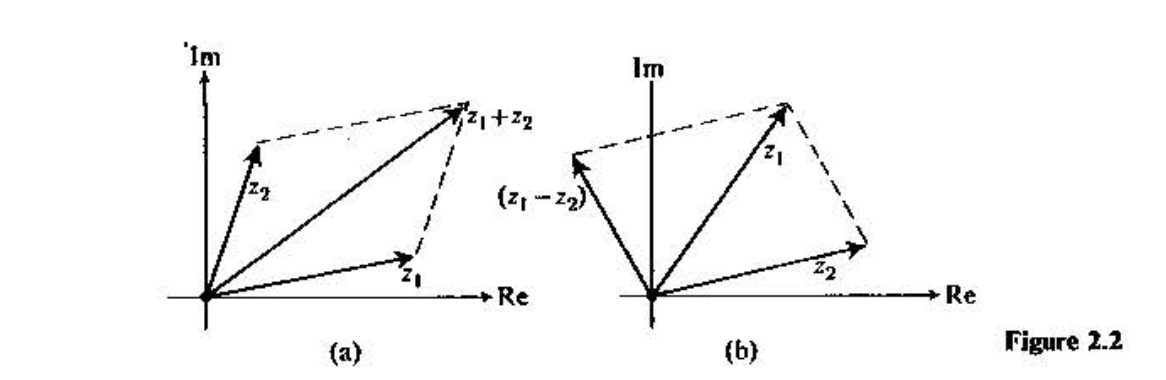
\includegraphics[width=0.75\textwidth]{images/parallelogram_rule.png}
    \caption{The parallelogram rule. (From Butkov.)}
    \label{fig:parallelogram_rule}
\end{figure}


\begin{enumerate}
    \item\mytag{recommended} Let $z = x + \rmi y \in \CC$. Illustrate the addition $w = z + \bar{z}$ in a coordinate system using the parallelogram rule.
    \item Recall our earlier exercise, where $\CC$ was regarded as the real vector space $\RR^2$. Let $z_i= x_i + \rmi y_i$, and denote the corresponding vectors in $\RR^2$ by $\bvec{v}_i$. Show that
    \begin{equation}
        \braket{\bvec{v}_1,\bvec{v}_2} = \Re (\overline{z_1} z_2) = \Re (z_1 \overline{z}_2).
    \end{equation}
    \item Another product in $\RR^2$ (and indeed $\RR^3$) is the \emph{cross product}:
    \begin{equation}
        \bvec{v}_1\times \bvec{v}_2 = \begin{vmatrix} v_{11} & v_{12} \\ v_{21} & v_{22} \end{vmatrix},
    \end{equation}
    the matrix determinant. Show that
    \begin{equation}
        \bvec{v}_1 \times \bvec{v}_2 = \Im (\overline{z_1} z_2) = -\Im (z_1 \overline{z}_2).
    \end{equation}
    \item Show that the function $z \mapsto \rmi z$ is a counterclockwise rotation by $\pi/2$. Find the function that performs a clockwise rotation by the same angle.
\end{enumerate}

\section{Complex functions}

\begin{solution}
{\bfseries Tutor note:} I think that this exercise is very nice. It is not too hard if the student has some experience with the equation $y'' = -y$.
\end{solution}
In this section, we give some relatively easy exercises to illustrate the important concepts of complex analytic functions.


\subsection{The complex exponential function}

In this exercise, we derive the complex exponential function. The starting point is the real exponential function, which is the unique function $f(x) = \exp(x)$ that satisfies
\begin{equation}
    f(x_1 + x_2) = f(x_1)f(x_2), \quad f(0) = 1.
\end{equation}
We desire to generalize $\exp(x)$ to the complex plane, so that $\exp(x + 0\rmi) = \exp(x) \in \RR$.

To avoid confusion, we call this unknown function $f : \CC \to \CC$.
\begin{enumerate}
    \item Show that $f(x + \rmi y) = \exp(x) f(\rmi y)$. (Thus, we need to determine $f(\rmi y)$.)
    \item We set $f(\rmi y) = A(y) + \rmi B(y)$. Show that 
    \begin{equation}
        A(y) =  B'(y), \quad B(y) = - A'(y),
    \end{equation}
    and hence that $A''(y) = -A(y)$. Hint: Cauchy--Riemann.
    \item The general solution to the ODE $A'' = -A$ is
    \begin{equation}
        A(y) = \alpha \cos(t) + \beta\sin(y),
    \end{equation}
    where $\alpha$ and $\beta$ are constants to be determined. Show that $\alpha = 1$ and $\beta = 0$ are the only constants compatible with $f(z)$ being a generalization of the real exponential function.
    \item Conclude that
    \begin{equation}
        f(x + \rmi y) = e^x(\cos y + \rmi \sin y)
    \end{equation}
    \item Show that $(\exp(z))' = \exp(z)$, using Cauchy--Riemann, and that $\exp(z)$ is everywhere analytic.
    \item Show that the equation
    \begin{equation}
        \exp(z) = w
    \end{equation}
    has infinitely many solutions for any $w\neq 0$.
    \item Show that $\exp(z) \neq 0$.
\end{enumerate}


\subsection{Taylor series}



\begin{enumerate}
    \item  Consider the Taylor series
    \begin{equation}
        \sum_{n=0}^\infty z^n  = 1 + z + z^2 + \ldots \longrightarrow \frac{1}{1-z}.
    \end{equation}
    Show that the $N$th partial sum is
    \begin{equation}
        \sum_{n=1}^{N} \frac{1 - z^{N+1}}{1 - z}.
    \end{equation}
    Here, the polynomial long division algorithm is useful.
    \item Find an upper bound for $|z|$ such that the partial sum converges to $1/(1-z)$.
    \item  The Taylor series for the exponential function is
    \begin{equation}
        \sum_{n=0}^\infty \frac{1}{n!} z^n.
    \end{equation}
    Using the definition of the complex exponential, find the Taylor series for $\cos(x)$ and $\sin(x)$, for $x\in\RR$.
    \item Make plots of the partial sums of the sine and cosine Taylor series to verify your result.
    \item Find the Taylor series for the function $f(z) = (e^z - 1)/z$
    \item Find the Taylor series for the function $f(z) = \sin(z)/z$ for $z\neq 0$ and $f(0) = 1$.
\end{enumerate}

\subsection{Singularities}

\begin{enumerate}
    \item \mytag{recommended} Consider the function $f(z) = \frac{1}{z(z-1)}$. How many poles does $f$ have, and where are they? What are the order of the poles? Can you write down the Laurent series of $f$ around $z=0$?
    \begin{solution}
    The poles are at $z=0$ and $z=1$, where the function blows up as $1/z$. Thus, the poles are of order 1. From the Taylor series of $1/(1-z)$ we see that
    \[ f(z) = z^{-1} + 1 + z + z^2 + \cdots \]
    \end{solution}
    \item Does the function $f(z) = 1/\sin(z)$ have a pole? Where? What order?
    \begin{solution}
    Taylor expansion of $\sin(z)$ shows that $f(z) \sim 1/z$ as $z\to 0$, so  the pole is of order $1$.
    \end{solution}
    \item Find the singularities of $f(z) = e^{-1/(z-1)^2}$.
    \begin{solution}
    The exponent has a pole at $z=1$ (of order 2). This means that the exponential function gives an essential singularity at $z=1$.
    \end{solution}
\end{enumerate}

\subsection{Line integrals}

Let 
\begin{equation}
    f(z)  = %\frac{1}{(z-1)(z-i)(z-1)} 
    %(z2 - 2z + 1)(z - i)
    %(z^3 - 2z^2 + z - iz^2 + 2iz - i)
    \frac{1}{z^3 - (2+\rmi)z^2 + (1 + 2\rmi)z - \rmi}
\end{equation} 
\begin{enumerate}
    \item Let $\Gamma_\epsilon(w)$ be the simple closed curve defined by the counter-clockwise border of the $\epsilon$-ball $B_\epsilon(w)$. Write down a parameterization (a path) for this curve.
    \begin{solution}
        $\gamma(t) = w + \epsilon e^{it}$, $0 \leq t < 2\pi$.  
    \end{solution}
    \item Identify the poles $P = \{w_1, w_2, \cdots \}$ of $f(z)$ and their order. Hint: A zero of the denominator is $z = \rmi$.
    \begin{solution}
        The denominator can be factorized as $(z-1)^2(z-\rmi)$, and therefore we have a pole of order 2 at $w_1 = 1$ and a pole of order 1 at $w_2 = \rmi$.
    \end{solution}
    \item What is the value of
    \begin{equation}
        \oint_{\Gamma_\epsilon(0)} f(z)\, \rmd z \quad \text{?}
    \end{equation}
    fpr $\epsilon = 1/2$?
    \begin{solution}
        The function has no poles inside the $\epsilon$-ball, so the integral is zero by Cauchy's integral theorem.
    \end{solution}
    \item Find the value for the line integrals, 
    \begin{equation}
        \oint_{\Gamma_\epsilon(w_i)} f(z) \, \rmd z,
    \end{equation}
    for $\epsilon=1/2$. Hint: Don't attempt the integral directly, but instead compute consider the Laurent series.
    It can be useful to use the Taylor expansion
    \begin{equation}
        \frac{1}{a - z} = \frac{1}{a} \frac{1}{1 - z/a} = \frac{1}{a} \sum_{n=0}^\infty (z/a)^n.
    \end{equation}
    \begin{solution}
        We know that the integral around the second-order pole is zero, since the path does not enclose any other pole. The only nonzero integral would be the one around the first-order pole $w = \rmi$. We compute the Laurent series around $w$. Write $z = \rmi + u$ where $u = e^{it}$ to be inserted later. Let $a = 1 - \rmi$.
        \[ f(\rmi + u) = \frac{1}{[(1-\rmi) - u]^2 u} = \frac{1}{a} \frac{1}{\hat{u}(1 - \hat{u})^2}, \quad \hat{u} = u/a. \]
        \[ \frac{1}{1-\hat{u}} = 1 + \hat{u} + \hat{u}^2 + \cdots \] 
        \[ \left(\frac{1}{1-\hat{u}}\right)^2 = 1 + 2\hat{u} + 2 \hat{u}^2 + 2\hat{u}^3 + \cdots \]
        \[ f(\rmi + u) = \frac{1}{a} (\hat{u}^{-1} + 2 + 2 \hat{u} + 2 \hat{u}^2 + \cdots\]
        Inserting back $\hat{u} = u/a$, we get the Laurent series around $w = \rmi$. Integrating aroud the loop will only give contributions from the $u^{-1}$ term; all the other terms are analytic inside the $\epsilon$-ball and give zero integrals.
        \[ \oint \frac{1}{a} \hat{u}^{-1} \rmd z = \oint z^{-1} \rmd z. \]
        Inserting the parameterization,
        \[ \rmi \int_0^{2\pi} e^{-\rmi t} e^{\rmi t} \rmd t = 2 \pi \rmi. \]
        Thus
        \[ \oint_{\Gamma_\epsilon(\rmi)} f(z) \, \rmd z = 2 \pi \rmi. \]
        
    \end{solution}
\end{enumerate}



\section{Complex step method}
\begin{solution}
{\bfseries Tutor note:} I think the tutors might be surprised by this exercise! I learned about the method only last year. This exercise is very nice, in my opinion. However, it may be a little advanced for some students, because it requires basic understanding of cancellation errors in floating point arithmetic.
\end{solution}

\mytag{for the curious}

Let $f(x)$ be a real-valued function, assumed to be analytic near some $x$, i.e., it agrees with its Taylor series in the vicinity of $x$. 
\begin{enumerate}
    \item Explain why there exists a complex analytic function near $x + 0\rmi $ that agrees with $f$ on the real axis.
    \begin{solution}
    The convergence radius of the real series is finite by assumption. Promoting the series to a complex series will give a convergent series with the same convergence radius. Hence, there is a unique complex analytic function that extends $f(x)$ into the complex plane near $x$. 
    \end{solution}
\end{enumerate}

A classical method for computing a numerical derivative of a $C^1$ function is the finite difference approximation:
\begin{equation}
    f'(x) \approx \delta_h f(x) := \frac{f(x+h) - f(x-h)}{2h}.
\end{equation}
The error is $\mathcal{O}(h^2)$.
In the rest of the exercise, let $f$ be given by
\begin{equation}
    f(x) = \exp(x),
\end{equation}
and we wish to differentiate around $x=1$.
\begin{enumerate}[resume]
    \item Write a small program that uses standard double precision floating point arithmetic to  compute the finite difference derivative for step lengths from the interval $h \in [10^{-9}, 10^{-1}]$.
    \item Make a plot of the absolute value of the error in the approximation as function of $h$. Use log scales. 
    \begin{solution}
    The student should observe that the accuracy deteriorates when $h$ becomes too small, around $10^{-7}$.
    \end{solution}
\end{enumerate}

The \emph{complex step method} utilizes complex analyticity to avoid the cancellation errors seen in the finite difference scheme. It relies on the function in question being implemented/implementable using complex arithmetic.
\begin{enumerate}[resume]
    \item Show that 
    \begin{equation}
    f(x + \rmi h) = f(x) + \rmi h f'(x) - \frac{1}{2}h^2 f''(x) - \frac{\rmi h^3}{6} f'''(x) + \mathcal{O}(h^4).
    \end{equation}
    \begin{solution}
    Just compute the Taylor series.
    \end{solution}
    \item Solve for $f'(x)$, and show that
    \begin{equation}
        f'(x) = \Im \frac{f(x + \rmi h)}{h} + \mathcal{O}(h^2).
    \end{equation}
    This is the complex step method.
    \begin{solution}
    The main observation is that the zeroth and second order terms are purely real, while the first and third are purely imaginary. The given approximation then eliminates the real parts, which explains the second-order error.
    \end{solution}
    \item In the plot from above, add a plot of the error of the complex step method. Compare.
    \begin{solution}
    The student should observe that the accuracy does \emph{not} deteriorate. This is because there is no cancellation errors in play -- the program simply computes a function value.
    \end{solution}
\end{enumerate}



\end{document}

